\documentclass[1p]{elsarticle_modified}
%\bibliographystyle{elsarticle-num}

%\usepackage[colorlinks]{hyperref}
%\usepackage{abbrmath_seonhwa} %\Abb, \Ascr, \Acal ,\Abf, \Afrak
\usepackage{amsfonts}
\usepackage{amssymb}
\usepackage{amsmath}
\usepackage{amsthm}
\usepackage{scalefnt}
\usepackage{amsbsy}
\usepackage{kotex}
\usepackage{caption}
\usepackage{subfig}
\usepackage{color}
\usepackage{graphicx}
\usepackage{xcolor} %% white, black, red, green, blue, cyan, magenta, yellow
\usepackage{float}
\usepackage{setspace}
\usepackage{hyperref}

\usepackage{tikz}
\usetikzlibrary{arrows}

\usepackage{multirow}
\usepackage{array} % fixed length table
\usepackage{hhline}

%%%%%%%%%%%%%%%%%%%%%
\makeatletter
\renewcommand*\env@matrix[1][\arraystretch]{%
	\edef\arraystretch{#1}%
	\hskip -\arraycolsep
	\let\@ifnextchar\new@ifnextchar
	\array{*\c@MaxMatrixCols c}}
\makeatother %https://tex.stackexchange.com/questions/14071/how-can-i-increase-the-line-spacing-in-a-matrix
%%%%%%%%%%%%%%%

\usepackage[normalem]{ulem}

\newcommand{\msout}[1]{\ifmmode\text{\sout{\ensuremath{#1}}}\else\sout{#1}\fi}
%SOURCE: \msout is \stkout macro in https://tex.stackexchange.com/questions/20609/strikeout-in-math-mode

\newcommand{\cancel}[1]{
	\ifmmode
	{\color{red}\msout{#1}}
	\else
	{\color{red}\sout{#1}}
	\fi
}

\newcommand{\add}[1]{
	{\color{blue}\uwave{#1}}
}

\newcommand{\replace}[2]{
	\ifmmode
	{\color{red}\msout{#1}}{\color{blue}\uwave{#2}}
	\else
	{\color{red}\sout{#1}}{\color{blue}\uwave{#2}}
	\fi
}

\newcommand{\Sol}{\mathcal{S}} %segment
\newcommand{\D}{D} %diagram
\newcommand{\A}{\mathcal{A}} %arc


%%%%%%%%%%%%%%%%%%%%%%%%%%%%%5 test

\def\sl{\operatorname{\textup{SL}}(2,\Cbb)}
\def\psl{\operatorname{\textup{PSL}}(2,\Cbb)}
\def\quan{\mkern 1mu \triangleright \mkern 1mu}

\theoremstyle{definition}
\newtheorem{thm}{Theorem}[section]
\newtheorem{prop}[thm]{Proposition}
\newtheorem{lem}[thm]{Lemma}
\newtheorem{ques}[thm]{Question}
\newtheorem{cor}[thm]{Corollary}
\newtheorem{defn}[thm]{Definition}
\newtheorem{exam}[thm]{Example}
\newtheorem{rmk}[thm]{Remark}
\newtheorem{alg}[thm]{Algorithm}

\newcommand{\I}{\sqrt{-1}}
\begin{document}

%\begin{frontmatter}
%
%\title{Boundary parabolic representations of knots up to 8 crossings}
%
%%% Group authors per affiliation:
%\author{Yunhi Cho} 
%\address{Department of Mathematics, University of Seoul, Seoul, Korea}
%\ead{yhcho@uos.ac.kr}
%
%
%\author{Seonhwa Kim} %\fnref{s_kim}}
%\address{Center for Geometry and Physics, Institute for Basic Science, Pohang, 37673, Korea}
%\ead{ryeona17@ibs.re.kr}
%
%\author{Hyuk Kim}
%\address{Department of Mathematical Sciences, Seoul National University, Seoul 08826, Korea}
%\ead{hyukkim@snu.ac.kr}
%
%\author{Seokbeom Yoon}
%\address{Department of Mathematical Sciences, Seoul National University, Seoul, 08826,  Korea}
%\ead{sbyoon15@snu.ac.kr}
%
%\begin{abstract}
%We find all boundary parabolic representation of knots up to 8 crossings.
%
%\end{abstract}
%\begin{keyword}
%    \MSC[2010] 57M25 
%\end{keyword}
%
%\end{frontmatter}

%\linenumbers
%\tableofcontents
%
\newcommand\colored[1]{\textcolor{white}{\rule[-0.35ex]{0.8em}{1.4ex}}\kern-0.8em\color{red} #1}%
%\newcommand\colored[1]{\textcolor{white}{ #1}\kern-2.17ex	\textcolor{white}{ #1}\kern-1.81ex	\textcolor{white}{ #1}\kern-2.15ex\color{red}#1	}

{\Large $\underline{12a_{0485}~(K12a_{0485})}$}

\setlength{\tabcolsep}{10pt}
\renewcommand{\arraystretch}{1.6}
\vspace{1cm}\begin{tabular}{m{100pt}>{\centering\arraybackslash}m{274pt}}
\multirow{5}{120pt}{
	\centering
	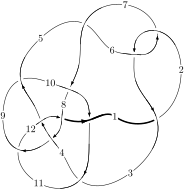
\includegraphics[width=112pt]{../../../GIT/diagram.site/Diagrams/png/1286_12a_0485.png}\\
\ \ \ A knot diagram\footnotemark}&
\allowdisplaybreaks
\textbf{Linearized knot diagam} \\
\cline{2-2}
 &
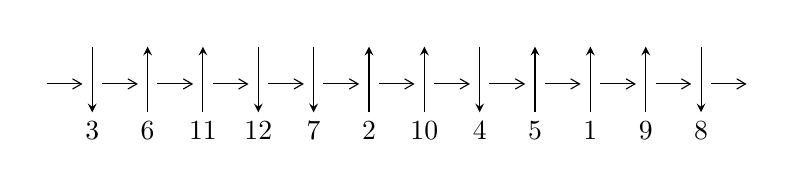
\begin{tikzpicture}[x=20pt, y=17pt]
	% nodes
	\node (C0) at (0, 0) {};
	\node (C1) at (1, 0) {};
	\node (C1U) at (1, +1) {};
	\node (C1D) at (1, -1) {3};

	\node (C2) at (2, 0) {};
	\node (C2U) at (2, +1) {};
	\node (C2D) at (2, -1) {6};

	\node (C3) at (3, 0) {};
	\node (C3U) at (3, +1) {};
	\node (C3D) at (3, -1) {11};

	\node (C4) at (4, 0) {};
	\node (C4U) at (4, +1) {};
	\node (C4D) at (4, -1) {12};

	\node (C5) at (5, 0) {};
	\node (C5U) at (5, +1) {};
	\node (C5D) at (5, -1) {7};

	\node (C6) at (6, 0) {};
	\node (C6U) at (6, +1) {};
	\node (C6D) at (6, -1) {2};

	\node (C7) at (7, 0) {};
	\node (C7U) at (7, +1) {};
	\node (C7D) at (7, -1) {10};

	\node (C8) at (8, 0) {};
	\node (C8U) at (8, +1) {};
	\node (C8D) at (8, -1) {4};

	\node (C9) at (9, 0) {};
	\node (C9U) at (9, +1) {};
	\node (C9D) at (9, -1) {5};

	\node (C10) at (10, 0) {};
	\node (C10U) at (10, +1) {};
	\node (C10D) at (10, -1) {1};

	\node (C11) at (11, 0) {};
	\node (C11U) at (11, +1) {};
	\node (C11D) at (11, -1) {9};

	\node (C12) at (12, 0) {};
	\node (C12U) at (12, +1) {};
	\node (C12D) at (12, -1) {8};
	\node (C13) at (13, 0) {};

	% arrows
	\draw[->,>={angle 60}]
	(C0) edge (C1) (C1) edge (C2) (C2) edge (C3) (C3) edge (C4) (C4) edge (C5) (C5) edge (C6) (C6) edge (C7) (C7) edge (C8) (C8) edge (C9) (C9) edge (C10) (C10) edge (C11) (C11) edge (C12) (C12) edge (C13) ;	\draw[->,>=stealth]
	(C1U) edge (C1D) (C2D) edge (C2U) (C3D) edge (C3U) (C4U) edge (C4D) (C5U) edge (C5D) (C6D) edge (C6U) (C7D) edge (C7U) (C8U) edge (C8D) (C9D) edge (C9U) (C10D) edge (C10U) (C11D) edge (C11U) (C12U) edge (C12D) ;
	\end{tikzpicture} \\
\hhline{~~} \\& 
\textbf{Solving Sequence} \\ \cline{2-2} 
 &
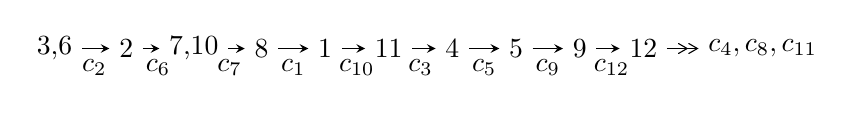
\begin{tikzpicture}[x=23pt, y=7pt]
	% node
	\node (A0) at (-1/8, 0) {3,6};
	\node (A1) at (1, 0) {2};
	\node (A2) at (33/16, 0) {7,10};
	\node (A3) at (25/8, 0) {8};
	\node (A4) at (33/8, 0) {1};
	\node (A5) at (41/8, 0) {11};
	\node (A6) at (49/8, 0) {4};
	\node (A7) at (57/8, 0) {5};
	\node (A8) at (65/8, 0) {9};
	\node (A9) at (73/8, 0) {12};
	\node (C1) at (1/2, -1) {$c_{2}$};
	\node (C2) at (3/2, -1) {$c_{6}$};
	\node (C3) at (21/8, -1) {$c_{7}$};
	\node (C4) at (29/8, -1) {$c_{1}$};
	\node (C5) at (37/8, -1) {$c_{10}$};
	\node (C6) at (45/8, -1) {$c_{3}$};
	\node (C7) at (53/8, -1) {$c_{5}$};
	\node (C8) at (61/8, -1) {$c_{9}$};
	\node (C9) at (69/8, -1) {$c_{12}$};
	\node (A10) at (11, 0) {$c_{4},c_{8},c_{11}$};

	% edge
	\draw[->,>=stealth]	
	(A0) edge (A1) (A1) edge (A2) (A2) edge (A3) (A3) edge (A4) (A4) edge (A5) (A5) edge (A6) (A6) edge (A7) (A7) edge (A8) (A8) edge (A9) ;
	\draw[->>,>={angle 60}]	
	(A9) edge (A10);
\end{tikzpicture} \\ 

\end{tabular} \\

\footnotetext{
The image of knot diagram is generated by the software ``\textbf{Draw programme}" developed by Andrew Bartholomew(\url{http://www.layer8.co.uk/maths/draw/index.htm\#Running-draw}), where we modified some parts for our purpose(\url{https://github.com/CATsTAILs/LinksPainter}).
}\phantom \\ \newline 
\centering \textbf{Ideals for irreducible components\footnotemark of $X_{\text{par}}$} 
 
\begin{align*}
I^u_{1}&=\langle 
192609591 u^{55}-2727061067 u^{54}+\cdots+14468204 b+16035728512,\\
\phantom{I^u_{1}}&\phantom{= \langle  }1002233032 u^{55}-8827487697 u^{54}+\cdots+14468204 a+16773966195,\;u^{56}-9 u^{55}+\cdots+36 u-16\rangle \\
I^u_{2}&=\langle 
5.06413\times10^{16} a^{3} u^{26}+2.15067\times10^{17} a^{2} u^{26}+\cdots-1.13428\times10^{19} a+9.45090\times10^{18},\\
\phantom{I^u_{2}}&\phantom{= \langle  }3 u^{26} a^3-9 u^{26} a^2+\cdots-25 a+21,\;u^{27}+2 u^{26}+\cdots-4 u^2-1\rangle \\
I^u_{3}&=\langle 
55 u^{28}-252 u^{27}+\cdots+21 b+61,\;61 u^{28}-189 u^{27}+\cdots+21 a-32,\;u^{29}-4 u^{28}+\cdots-6 u^2-1\rangle \\
I^u_{4}&=\langle 
a u+b-1,\;a^2+a u+a+1,\;u^2+u+1\rangle \\
I^u_{5}&=\langle 
a u+b- u,\;a^2- a- u-1,\;u^2+u+1\rangle \\
\\
\end{align*}
\raggedright * 5 irreducible components of $\dim_{\mathbb{C}}=0$, with total 201 representations.\\
\footnotetext{All coefficients of polynomials are rational numbers. But the coefficients are sometimes approximated in decimal forms when there is not enough margin.}
\newpage
\renewcommand{\arraystretch}{1}
\centering \section*{I. $I^u_{1}= \langle 1.93\times10^{8} u^{55}-2.73\times10^{9} u^{54}+\cdots+1.45\times10^{7} b+1.60\times10^{10},\;1.00\times10^{9} u^{55}-8.83\times10^{9} u^{54}+\cdots+1.45\times10^{7} a+1.68\times10^{10},\;u^{56}-9 u^{55}+\cdots+36 u-16 \rangle$}
\flushleft \textbf{(i) Arc colorings}\\
\begin{tabular}{m{7pt} m{180pt} m{7pt} m{180pt} }
\flushright $a_{3}=$&$\begin{pmatrix}1\\0\end{pmatrix}$ \\
\flushright $a_{6}=$&$\begin{pmatrix}0\\u\end{pmatrix}$ \\
\flushright $a_{2}=$&$\begin{pmatrix}1\\u^2\end{pmatrix}$ \\
\flushright $a_{7}=$&$\begin{pmatrix}u\\u^3+u\end{pmatrix}$ \\
\flushright $a_{10}=$&$\begin{pmatrix}-69.2714 u^{55}+610.130 u^{54}+\cdots+2096.44 u-1159.37\\-13.3126 u^{55}+188.486 u^{54}+\cdots+1334.40 u-1108.34\end{pmatrix}$ \\
\flushright $a_{8}=$&$\begin{pmatrix}-8.78193 u^{55}+253.245 u^{54}+\cdots+2714.47 u-2326.29\\174.208 u^{55}-1303.60 u^{54}+\cdots-2009.14 u-140.511\end{pmatrix}$ \\
\flushright $a_{1}=$&$\begin{pmatrix}u^2+1\\u^2\end{pmatrix}$ \\
\flushright $a_{11}=$&$\begin{pmatrix}-20.3141 u^{55}+164.851 u^{54}+\cdots+477.918 u-272.674\\-4.39070 u^{55}+60.8214 u^{54}+\cdots+437.619 u-425.076\end{pmatrix}$ \\
\flushright $a_{4}=$&$\begin{pmatrix}79.7522 u^{55}-623.369 u^{54}+\cdots-1262.96 u+253.754\\100.284 u^{55}-911.993 u^{54}+\cdots-3411.74 u+1923.40\end{pmatrix}$ \\
\flushright $a_{5}=$&$\begin{pmatrix}u^3\\u^5+u^3+u\end{pmatrix}$ \\
\flushright $a_{9}=$&$\begin{pmatrix}-31.3270 u^{55}+292.918 u^{54}+\cdots+1098.99 u-564.552\\41.0305 u^{55}-290.047 u^{54}+\cdots-197.308 u-195.175\end{pmatrix}$ \\
\flushright $a_{12}=$&$\begin{pmatrix}-32.0066 u^{55}+315.058 u^{54}+\cdots+1431.56 u-896.451\\66.8287 u^{55}-495.324 u^{54}+\cdots-647.072 u-154.409\end{pmatrix}$\\&\end{tabular}
\flushleft \textbf{(ii) Obstruction class $= -1$}\\~\\
\flushleft \textbf{(iii) Cusp Shapes $= -\frac{1195774015}{3617051} u^{55}+\frac{10894419483}{3617051} u^{54}+\cdots+\frac{40309490750}{3617051} u-\frac{22849509610}{3617051}$}\\~\\
\newpage\renewcommand{\arraystretch}{1}
\flushleft \textbf{(iv) u-Polynomials at the component}\newline \\
\begin{tabular}{m{50pt}|m{274pt}}
Crossings & \hspace{64pt}u-Polynomials at each crossing \\
\hline $$\begin{aligned}c_{1},c_{5}\end{aligned}$$&$\begin{aligned}
&u^{56}+17 u^{55}+\cdots+2640 u+256
\end{aligned}$\\
\hline $$\begin{aligned}c_{2},c_{6}\end{aligned}$$&$\begin{aligned}
&u^{56}-9 u^{55}+\cdots+36 u-16
\end{aligned}$\\
\hline $$\begin{aligned}c_{3},c_{9}\end{aligned}$$&$\begin{aligned}
&u^{56}- u^{55}+\cdots+166 u+34
\end{aligned}$\\
\hline $$\begin{aligned}c_{4},c_{8}\end{aligned}$$&$\begin{aligned}
&u^{56}-5 u^{54}+\cdots+u-1
\end{aligned}$\\
\hline $$\begin{aligned}c_{7},c_{10}\end{aligned}$$&$\begin{aligned}
&u^{56}- u^{55}+\cdots-21 u+1
\end{aligned}$\\
\hline $$\begin{aligned}c_{11}\end{aligned}$$&$\begin{aligned}
&u^{56}+43 u^{55}+\cdots-34 u-4
\end{aligned}$\\
\hline $$\begin{aligned}c_{12}\end{aligned}$$&$\begin{aligned}
&u^{56}+53 u^{55}+\cdots-738197504 u-33554432
\end{aligned}$\\
\hline
\end{tabular}\\~\\
\newpage\renewcommand{\arraystretch}{1}
\flushleft \textbf{(v) Riley Polynomials at the component}\newline \\
\begin{tabular}{m{50pt}|m{274pt}}
Crossings & \hspace{64pt}Riley Polynomials at each crossing \\
\hline $$\begin{aligned}c_{1},c_{5}\end{aligned}$$&$\begin{aligned}
&y^{56}+45 y^{55}+\cdots-636672 y+65536
\end{aligned}$\\
\hline $$\begin{aligned}c_{2},c_{6}\end{aligned}$$&$\begin{aligned}
&y^{56}+17 y^{55}+\cdots+2640 y+256
\end{aligned}$\\
\hline $$\begin{aligned}c_{3},c_{9}\end{aligned}$$&$\begin{aligned}
&y^{56}-31 y^{55}+\cdots-9332 y+1156
\end{aligned}$\\
\hline $$\begin{aligned}c_{4},c_{8}\end{aligned}$$&$\begin{aligned}
&y^{56}-10 y^{55}+\cdots-9 y+1
\end{aligned}$\\
\hline $$\begin{aligned}c_{7},c_{10}\end{aligned}$$&$\begin{aligned}
&y^{56}-7 y^{55}+\cdots-45 y+1
\end{aligned}$\\
\hline $$\begin{aligned}c_{11}\end{aligned}$$&$\begin{aligned}
&y^{56}-21 y^{55}+\cdots-508 y+16
\end{aligned}$\\
\hline $$\begin{aligned}c_{12}\end{aligned}$$&$\begin{aligned}
&y^{56}-9 y^{55}+\cdots+19140298416324608 y+1125899906842624
\end{aligned}$\\
\hline
\end{tabular}\\~\\
\newpage\flushleft \textbf{(vi) Complex Volumes and Cusp Shapes}
$$\begin{array}{c|c|c}  
\text{Solutions to }I^u_{1}& \I (\text{vol} + \sqrt{-1}CS) & \text{Cusp shape}\\
 \hline 
\begin{aligned}
u &= -0.148611 + 0.987288 I \\
a &= -0.105326 + 0.776858 I \\
b &= -0.751329 - 0.219436 I\end{aligned}
 & -5.08582 - 0.04483 I & \phantom{-0.000000 } 0 \\ \hline\begin{aligned}
u &= -0.148611 - 0.987288 I \\
a &= -0.105326 - 0.776858 I \\
b &= -0.751329 + 0.219436 I\end{aligned}
 & -5.08582 + 0.04483 I & \phantom{-0.000000 } 0 \\ \hline\begin{aligned}
u &= -1.02530\phantom{ +0.000000I} \\
a &= -0.206826\phantom{ +0.000000I} \\
b &= \phantom{-}0.212059\phantom{ +0.000000I}\end{aligned}
 & \phantom{-}1.23312\phantom{ +0.000000I} & \phantom{-}12.2390\phantom{ +0.000000I} \\ \hline\begin{aligned}
u &= -0.388031 + 0.964876 I \\
a &= -0.013054 - 0.703235 I \\
b &= \phantom{-}0.683600 + 0.260282 I\end{aligned}
 & \phantom{-}0.66649 - 6.36541 I & \phantom{-0.000000 } 0 \\ \hline\begin{aligned}
u &= -0.388031 - 0.964876 I \\
a &= -0.013054 + 0.703235 I \\
b &= \phantom{-}0.683600 - 0.260282 I\end{aligned}
 & \phantom{-}0.66649 + 6.36541 I & \phantom{-0.000000 } 0 \\ \hline\begin{aligned}
u &= \phantom{-}0.754659 + 0.782525 I \\
a &= \phantom{-}1.31638 + 1.21329 I \\
b &= \phantom{-}0.04399 + 1.94571 I\end{aligned}
 & \phantom{-}0.734279 + 0.907581 I & \phantom{-0.000000 } 0 \\ \hline\begin{aligned}
u &= \phantom{-}0.754659 - 0.782525 I \\
a &= \phantom{-}1.31638 - 1.21329 I \\
b &= \phantom{-}0.04399 - 1.94571 I\end{aligned}
 & \phantom{-}0.734279 - 0.907581 I & \phantom{-0.000000 } 0 \\ \hline\begin{aligned}
u &= \phantom{-}0.410147 + 0.807610 I \\
a &= \phantom{-}0.503137 + 0.296621 I \\
b &= -0.033194 + 0.527996 I\end{aligned}
 & -0.05668 + 1.76377 I & \phantom{-0.000000 } 0. - 5.48632 I \\ \hline\begin{aligned}
u &= \phantom{-}0.410147 - 0.807610 I \\
a &= \phantom{-}0.503137 - 0.296621 I \\
b &= -0.033194 - 0.527996 I\end{aligned}
 & -0.05668 - 1.76377 I & \phantom{-0.000000 -}0. + 5.48632 I \\ \hline\begin{aligned}
u &= -0.461995 + 1.015350 I \\
a &= -0.277333 - 0.297378 I \\
b &= \phantom{-}0.430069 - 0.144203 I\end{aligned}
 & -3.28970 - 5.83406 I & \phantom{-0.000000 } 0\\
 \hline 
 \end{array}$$\newpage$$\begin{array}{c|c|c}  
\text{Solutions to }I^u_{1}& \I (\text{vol} + \sqrt{-1}CS) & \text{Cusp shape}\\
 \hline 
\begin{aligned}
u &= -0.461995 - 1.015350 I \\
a &= -0.277333 + 0.297378 I \\
b &= \phantom{-}0.430069 + 0.144203 I\end{aligned}
 & -3.28970 + 5.83406 I & \phantom{-0.000000 } 0 \\ \hline\begin{aligned}
u &= \phantom{-}0.732257 + 0.863189 I \\
a &= -0.56605 - 2.39805 I \\
b &= \phantom{-}1.65547 - 2.24459 I\end{aligned}
 & \phantom{-}2.80607 + 4.77645 I & \phantom{-0.000000 } 0 \\ \hline\begin{aligned}
u &= \phantom{-}0.732257 - 0.863189 I \\
a &= -0.56605 + 2.39805 I \\
b &= \phantom{-}1.65547 + 2.24459 I\end{aligned}
 & \phantom{-}2.80607 - 4.77645 I & \phantom{-0.000000 } 0 \\ \hline\begin{aligned}
u &= \phantom{-}0.090367 + 0.856778 I \\
a &= \phantom{-}0.141600 + 0.932125 I \\
b &= -0.785828 + 0.205553 I\end{aligned}
 & -1.45441 + 1.82954 I & -3.97315 - 5.04709 I \\ \hline\begin{aligned}
u &= \phantom{-}0.090367 - 0.856778 I \\
a &= \phantom{-}0.141600 - 0.932125 I \\
b &= -0.785828 - 0.205553 I\end{aligned}
 & -1.45441 - 1.82954 I & -3.97315 + 5.04709 I \\ \hline\begin{aligned}
u &= \phantom{-}0.721081 + 0.885164 I \\
a &= -2.05381 - 0.72427 I \\
b &= -0.83986 - 2.34021 I\end{aligned}
 & \phantom{-}2.73433 + 0.76799 I & \phantom{-0.000000 } 0 \\ \hline\begin{aligned}
u &= \phantom{-}0.721081 - 0.885164 I \\
a &= -2.05381 + 0.72427 I \\
b &= -0.83986 + 2.34021 I\end{aligned}
 & \phantom{-}2.73433 - 0.76799 I & \phantom{-0.000000 } 0 \\ \hline\begin{aligned}
u &= -0.847184 + 0.024271 I \\
a &= \phantom{-}0.512339 + 0.300014 I \\
b &= -0.441327 - 0.241732 I\end{aligned}
 & \phantom{-}5.35540 + 10.65240 I & \phantom{-}8.10098 - 7.27900 I \\ \hline\begin{aligned}
u &= -0.847184 - 0.024271 I \\
a &= \phantom{-}0.512339 - 0.300014 I \\
b &= -0.441327 + 0.241732 I\end{aligned}
 & \phantom{-}5.35540 - 10.65240 I & \phantom{-}8.10098 + 7.27900 I \\ \hline\begin{aligned}
u &= -0.756418 + 0.870995 I \\
a &= \phantom{-}0.472676 + 0.001674 I \\
b &= -0.358999 + 0.410431 I\end{aligned}
 & \phantom{-}3.13677 - 0.64477 I & \phantom{-0.000000 } 0\\
 \hline 
 \end{array}$$\newpage$$\begin{array}{c|c|c}  
\text{Solutions to }I^u_{1}& \I (\text{vol} + \sqrt{-1}CS) & \text{Cusp shape}\\
 \hline 
\begin{aligned}
u &= -0.756418 - 0.870995 I \\
a &= \phantom{-}0.472676 - 0.001674 I \\
b &= -0.358999 - 0.410431 I\end{aligned}
 & \phantom{-}3.13677 + 0.64477 I & \phantom{-0.000000 } 0 \\ \hline\begin{aligned}
u &= -0.315267 + 1.117870 I \\
a &= -0.325563 + 0.574726 I \\
b &= -0.539830 - 0.545129 I\end{aligned}
 & \phantom{-}1.6611 - 14.5883 I & \phantom{-0.000000 } 0 \\ \hline\begin{aligned}
u &= -0.315267 - 1.117870 I \\
a &= -0.325563 - 0.574726 I \\
b &= -0.539830 + 0.545129 I\end{aligned}
 & \phantom{-}1.6611 + 14.5883 I & \phantom{-0.000000 } 0 \\ \hline\begin{aligned}
u &= -0.752842 + 0.890277 I \\
a &= -0.412632 - 0.169367 I \\
b &= \phantom{-}0.461431 - 0.239850 I\end{aligned}
 & \phantom{-}3.07720 - 5.07348 I & \phantom{-0.000000 } 0 \\ \hline\begin{aligned}
u &= -0.752842 - 0.890277 I \\
a &= -0.412632 + 0.169367 I \\
b &= \phantom{-}0.461431 + 0.239850 I\end{aligned}
 & \phantom{-}3.07720 + 5.07348 I & \phantom{-0.000000 } 0 \\ \hline\begin{aligned}
u &= \phantom{-}0.910217 + 0.748706 I \\
a &= \phantom{-}1.46008 + 1.53528 I \\
b &= \phantom{-}0.17952 + 2.49061 I\end{aligned}
 & \phantom{-}9.9171 - 14.1482 I & \phantom{-0.000000 } 0 \\ \hline\begin{aligned}
u &= \phantom{-}0.910217 - 0.748706 I \\
a &= \phantom{-}1.46008 - 1.53528 I \\
b &= \phantom{-}0.17952 - 2.49061 I\end{aligned}
 & \phantom{-}9.9171 + 14.1482 I & \phantom{-0.000000 } 0 \\ \hline\begin{aligned}
u &= -0.265751 + 1.169400 I \\
a &= -0.415551 - 0.112866 I \\
b &= \phantom{-}0.242420 - 0.455953 I\end{aligned}
 & \phantom{-}1.27517 + 6.83332 I & \phantom{-0.000000 } 0 \\ \hline\begin{aligned}
u &= -0.265751 - 1.169400 I \\
a &= -0.415551 + 0.112866 I \\
b &= \phantom{-}0.242420 + 0.455953 I\end{aligned}
 & \phantom{-}1.27517 - 6.83332 I & \phantom{-0.000000 } 0 \\ \hline\begin{aligned}
u &= \phantom{-}0.734138 + 0.954130 I \\
a &= \phantom{-}0.96728 + 1.64674 I \\
b &= -0.86109 + 2.13185 I\end{aligned}
 & \phantom{-}0.21426 + 4.75574 I & \phantom{-0.000000 } 0\\
 \hline 
 \end{array}$$\newpage$$\begin{array}{c|c|c}  
\text{Solutions to }I^u_{1}& \I (\text{vol} + \sqrt{-1}CS) & \text{Cusp shape}\\
 \hline 
\begin{aligned}
u &= \phantom{-}0.734138 - 0.954130 I \\
a &= \phantom{-}0.96728 - 1.64674 I \\
b &= -0.86109 - 2.13185 I\end{aligned}
 & \phantom{-}0.21426 - 4.75574 I & \phantom{-0.000000 } 0 \\ \hline\begin{aligned}
u &= \phantom{-}0.893467 + 0.810104 I \\
a &= -1.68903 - 1.19547 I \\
b &= -0.54064 - 2.43639 I\end{aligned}
 & \phantom{-}8.95532 - 4.37769 I & \phantom{-0.000000 } 0 \\ \hline\begin{aligned}
u &= \phantom{-}0.893467 - 0.810104 I \\
a &= -1.68903 + 1.19547 I \\
b &= -0.54064 + 2.43639 I\end{aligned}
 & \phantom{-}8.95532 + 4.37769 I & \phantom{-0.000000 } 0 \\ \hline\begin{aligned}
u &= \phantom{-}0.942592 + 0.754576 I \\
a &= \phantom{-}0.312382 + 1.175130 I \\
b &= -0.59227 + 1.34338 I\end{aligned}
 & \phantom{-}9.79014 + 6.70793 I & \phantom{-0.000000 } 0 \\ \hline\begin{aligned}
u &= \phantom{-}0.942592 - 0.754576 I \\
a &= \phantom{-}0.312382 - 1.175130 I \\
b &= -0.59227 - 1.34338 I\end{aligned}
 & \phantom{-}9.79014 - 6.70793 I & \phantom{-0.000000 } 0 \\ \hline\begin{aligned}
u &= -0.701393 + 0.337884 I \\
a &= -0.066176 - 0.592967 I \\
b &= \phantom{-}0.246769 + 0.393543 I\end{aligned}
 & \phantom{-}2.79814 + 2.42669 I & \phantom{-}7.0112 - 14.0897 I \\ \hline\begin{aligned}
u &= -0.701393 - 0.337884 I \\
a &= -0.066176 + 0.592967 I \\
b &= \phantom{-}0.246769 - 0.393543 I\end{aligned}
 & \phantom{-}2.79814 - 2.42669 I & \phantom{-}7.0112 + 14.0897 I \\ \hline\begin{aligned}
u &= \phantom{-}0.953287 + 0.766830 I \\
a &= -0.948615 - 0.800138 I \\
b &= -0.29073 - 1.49019 I\end{aligned}
 & \phantom{-}6.49118 - 4.87375 I & \phantom{-0.000000 } 0 \\ \hline\begin{aligned}
u &= \phantom{-}0.953287 - 0.766830 I \\
a &= -0.948615 + 0.800138 I \\
b &= -0.29073 + 1.49019 I\end{aligned}
 & \phantom{-}6.49118 + 4.87375 I & \phantom{-0.000000 } 0 \\ \hline\begin{aligned}
u &= \phantom{-}0.013411 + 0.744426 I \\
a &= \phantom{-}0.17390 - 1.95972 I \\
b &= \phantom{-}1.46120 + 0.10317 I\end{aligned}
 & -1.08652 - 1.99360 I & -2.94814 + 3.49725 I\\
 \hline 
 \end{array}$$\newpage$$\begin{array}{c|c|c}  
\text{Solutions to }I^u_{1}& \I (\text{vol} + \sqrt{-1}CS) & \text{Cusp shape}\\
 \hline 
\begin{aligned}
u &= \phantom{-}0.013411 - 0.744426 I \\
a &= \phantom{-}0.17390 + 1.95972 I \\
b &= \phantom{-}1.46120 - 0.10317 I\end{aligned}
 & -1.08652 + 1.99360 I & -2.94814 - 3.49725 I \\ \hline\begin{aligned}
u &= \phantom{-}0.814580 + 0.991484 I \\
a &= -0.94091 - 1.96051 I \\
b &= \phantom{-}1.17737 - 2.52990 I\end{aligned}
 & \phantom{-}8.37962 + 10.69940 I & \phantom{-0.000000 } 0 \\ \hline\begin{aligned}
u &= \phantom{-}0.814580 - 0.991484 I \\
a &= -0.94091 + 1.96051 I \\
b &= \phantom{-}1.17737 + 2.52990 I\end{aligned}
 & \phantom{-}8.37962 - 10.69940 I & \phantom{-0.000000 } 0 \\ \hline\begin{aligned}
u &= \phantom{-}0.792855 + 1.029230 I \\
a &= \phantom{-}1.25881 + 1.77766 I \\
b &= -0.83157 + 2.70503 I\end{aligned}
 & \phantom{-}9.0363 + 20.4388 I & \phantom{-0.000000 } 0 \\ \hline\begin{aligned}
u &= \phantom{-}0.792855 - 1.029230 I \\
a &= \phantom{-}1.25881 - 1.77766 I \\
b &= -0.83157 - 2.70503 I\end{aligned}
 & \phantom{-}9.0363 - 20.4388 I & \phantom{-0.000000 } 0 \\ \hline\begin{aligned}
u &= -0.112713 + 0.673401 I \\
a &= \phantom{-}1.041970 + 0.476281 I \\
b &= -0.438172 + 0.647982 I\end{aligned}
 & -0.99942 + 1.87855 I & -2.67770 - 3.80115 I \\ \hline\begin{aligned}
u &= -0.112713 - 0.673401 I \\
a &= \phantom{-}1.041970 - 0.476281 I \\
b &= -0.438172 - 0.647982 I\end{aligned}
 & -0.99942 - 1.87855 I & -2.67770 + 3.80115 I \\ \hline\begin{aligned}
u &= \phantom{-}0.819918 + 1.039760 I \\
a &= -0.595172 - 1.238170 I \\
b &= \phantom{-}0.79940 - 1.63403 I\end{aligned}
 & \phantom{-}5.61955 + 11.37810 I & \phantom{-0.000000 } 0 \\ \hline\begin{aligned}
u &= \phantom{-}0.819918 - 1.039760 I \\
a &= -0.595172 + 1.238170 I \\
b &= \phantom{-}0.79940 + 1.63403 I\end{aligned}
 & \phantom{-}5.61955 - 11.37810 I & \phantom{-0.000000 } 0 \\ \hline\begin{aligned}
u &= \phantom{-}0.820110 + 1.044490 I \\
a &= \phantom{-}0.919908 + 0.618661 I \\
b &= \phantom{-}0.10824 + 1.46820 I\end{aligned}
 & \phantom{-}8.88440 - 0.23202 I & \phantom{-0.000000 } 0\\
 \hline 
 \end{array}$$\newpage$$\begin{array}{c|c|c}  
\text{Solutions to }I^u_{1}& \I (\text{vol} + \sqrt{-1}CS) & \text{Cusp shape}\\
 \hline 
\begin{aligned}
u &= \phantom{-}0.820110 - 1.044490 I \\
a &= \phantom{-}0.919908 - 0.618661 I \\
b &= \phantom{-}0.10824 - 1.46820 I\end{aligned}
 & \phantom{-}8.88440 + 0.23202 I & \phantom{-0.000000 } 0 \\ \hline\begin{aligned}
u &= -0.406216 + 1.276320 I \\
a &= \phantom{-}0.102721 - 0.123005 I \\
b &= \phantom{-}0.115267 + 0.181071 I\end{aligned}
 & -3.08574 - 4.97156 I & \phantom{-0.000000 } 0 \\ \hline\begin{aligned}
u &= -0.406216 - 1.276320 I \\
a &= \phantom{-}0.102721 + 0.123005 I \\
b &= \phantom{-}0.115267 - 0.181071 I\end{aligned}
 & -3.08574 + 4.97156 I & \phantom{-0.000000 } 0 \\ \hline\begin{aligned}
u &= -0.541789 + 0.332536 I \\
a &= \phantom{-}0.584596 - 0.319325 I \\
b &= -0.210541 + 0.367406 I\end{aligned}
 & -1.37335 + 1.75176 I & -0.47779 - 2.41051 I \\ \hline\begin{aligned}
u &= -0.541789 - 0.332536 I \\
a &= \phantom{-}0.584596 + 0.319325 I \\
b &= -0.210541 - 0.367406 I\end{aligned}
 & -1.37335 - 1.75176 I & -0.47779 + 2.41051 I \\ \hline\begin{aligned}
u &= \phantom{-}0.615547\phantom{ +0.000000I} \\
a &= \phantom{-}0.989696\phantom{ +0.000000I} \\
b &= \phantom{-}0.609204\phantom{ +0.000000I}\end{aligned}
 & \phantom{-}1.54329\phantom{ +0.000000I} & \phantom{-}8.12550\phantom{ +0.000000I}\\
 \hline 
 \end{array}$$\newpage\newpage\renewcommand{\arraystretch}{1}
\centering \section*{II. $I^u_{2}= \langle 5.06\times10^{16} a^{3} u^{26}+2.15\times10^{17} a^{2} u^{26}+\cdots-1.13\times10^{19} a+9.45\times10^{18},\;3 u^{26} a^3-9 u^{26} a^2+\cdots-25 a+21,\;u^{27}+2 u^{26}+\cdots-4 u^2-1 \rangle$}
\flushleft \textbf{(i) Arc colorings}\\
\begin{tabular}{m{7pt} m{180pt} m{7pt} m{180pt} }
\flushright $a_{3}=$&$\begin{pmatrix}1\\0\end{pmatrix}$ \\
\flushright $a_{6}=$&$\begin{pmatrix}0\\u\end{pmatrix}$ \\
\flushright $a_{2}=$&$\begin{pmatrix}1\\u^2\end{pmatrix}$ \\
\flushright $a_{7}=$&$\begin{pmatrix}u\\u^3+u\end{pmatrix}$ \\
\flushright $a_{10}=$&$\begin{pmatrix}a\\-0.0194228 a^{3} u^{26}-0.0824861 a^{2} u^{26}+\cdots+4.35040 a-3.62477\end{pmatrix}$ \\
\flushright $a_{8}=$&$\begin{pmatrix}0.222877 a^{3} u^{26}-0.426660 a^{2} u^{26}+\cdots+0.709576 a+1.18860\\-0.175602 a^{3} u^{26}+0.512669 a^{2} u^{26}+\cdots-0.00724059 a-1.52161\end{pmatrix}$ \\
\flushright $a_{1}=$&$\begin{pmatrix}u^2+1\\u^2\end{pmatrix}$ \\
\flushright $a_{11}=$&$\begin{pmatrix}0.356153 a^{3} u^{26}+0.437054 a^{2} u^{26}+\cdots+3.71412 a-0.591491\\-0.0341233 a^{3} u^{26}+0.112725 a^{2} u^{26}+\cdots+3.57675 a-2.25136\end{pmatrix}$ \\
\flushright $a_{4}=$&$\begin{pmatrix}-0.777942 a^{3} u^{26}+0.215725 a^{2} u^{26}+\cdots-2.73581 a+3.08163\\0.0221625 a^{3} u^{26}+0.670679 a^{2} u^{26}+\cdots+1.24922 a-2.25944\end{pmatrix}$ \\
\flushright $a_{5}=$&$\begin{pmatrix}u^3\\u^5+u^3+u\end{pmatrix}$ \\
\flushright $a_{9}=$&$\begin{pmatrix}-0.402197 a^{3} u^{26}+0.289264 a^{2} u^{26}+\cdots+1.48602 a+1.29020\\0.356960 a^{3} u^{26}+0.574655 a^{2} u^{26}+\cdots+4.05346 a-3.72719\end{pmatrix}$ \\
\flushright $a_{12}=$&$\begin{pmatrix}0.324083 a^{3} u^{26}+0.0222001 a^{2} u^{26}+\cdots+5.02261 a-1.76900\\-0.0803756 a^{3} u^{26}-1.11721 a^{2} u^{26}+\cdots-1.52529 a+5.87076\end{pmatrix}$\\&\end{tabular}
\flushleft \textbf{(ii) Obstruction class $= -1$}\\~\\
\flushleft \textbf{(iii) Cusp Shapes $= -\frac{5409149913549089364}{2607312645830463659} u^{26} a^3+\frac{584973825734070008}{2607312645830463659} u^{26} a^2+\cdots+\frac{12887390798361837140}{2607312645830463659} a+\frac{898974269192559217}{2607312645830463659}$}\\~\\
\newpage\renewcommand{\arraystretch}{1}
\flushleft \textbf{(iv) u-Polynomials at the component}\newline \\
\begin{tabular}{m{50pt}|m{274pt}}
Crossings & \hspace{64pt}u-Polynomials at each crossing \\
\hline $$\begin{aligned}c_{1},c_{5}\end{aligned}$$&$\begin{aligned}
&(u^{27}+8 u^{26}+\cdots-8 u-1)^{4}
\end{aligned}$\\
\hline $$\begin{aligned}c_{2},c_{6}\end{aligned}$$&$\begin{aligned}
&(u^{27}+2 u^{26}+\cdots-4 u^2-1)^{4}
\end{aligned}$\\
\hline $$\begin{aligned}c_{3},c_{9}\end{aligned}$$&$\begin{aligned}
&u^{108}+2 u^{107}+\cdots+53770489 u+615212329
\end{aligned}$\\
\hline $$\begin{aligned}c_{4},c_{8}\end{aligned}$$&$\begin{aligned}
&u^{108}+4 u^{107}+\cdots+u+1
\end{aligned}$\\
\hline $$\begin{aligned}c_{7},c_{10}\end{aligned}$$&$\begin{aligned}
&u^{108}-5 u^{107}+\cdots-770948 u+186859
\end{aligned}$\\
\hline $$\begin{aligned}c_{11}\end{aligned}$$&$\begin{aligned}
&(u^{27}-13 u^{26}+\cdots-10 u+4)^{4}
\end{aligned}$\\
\hline $$\begin{aligned}c_{12}\end{aligned}$$&$\begin{aligned}
&(u^2- u+1)^{54}
\end{aligned}$\\
\hline
\end{tabular}\\~\\
\newpage\renewcommand{\arraystretch}{1}
\flushleft \textbf{(v) Riley Polynomials at the component}\newline \\
\begin{tabular}{m{50pt}|m{274pt}}
Crossings & \hspace{64pt}Riley Polynomials at each crossing \\
\hline $$\begin{aligned}c_{1},c_{5}\end{aligned}$$&$\begin{aligned}
&(y^{27}+24 y^{26}+\cdots-12 y-1)^{4}
\end{aligned}$\\
\hline $$\begin{aligned}c_{2},c_{6}\end{aligned}$$&$\begin{aligned}
&(y^{27}+8 y^{26}+\cdots-8 y-1)^{4}
\end{aligned}$\\
\hline $$\begin{aligned}c_{3},c_{9}\end{aligned}$$&$\begin{aligned}
&y^{108}-58 y^{107}+\cdots-1.51\times10^{19} y+3.78\times10^{17}
\end{aligned}$\\
\hline $$\begin{aligned}c_{4},c_{8}\end{aligned}$$&$\begin{aligned}
&y^{108}+34 y^{107}+\cdots+539 y+1
\end{aligned}$\\
\hline $$\begin{aligned}c_{7},c_{10}\end{aligned}$$&$\begin{aligned}
&y^{108}-53 y^{107}+\cdots-468863324560 y+34916285881
\end{aligned}$\\
\hline $$\begin{aligned}c_{11}\end{aligned}$$&$\begin{aligned}
&(y^{27}-5 y^{26}+\cdots+236 y-16)^{4}
\end{aligned}$\\
\hline $$\begin{aligned}c_{12}\end{aligned}$$&$\begin{aligned}
&(y^2+y+1)^{54}
\end{aligned}$\\
\hline
\end{tabular}\\~\\
\newpage\flushleft \textbf{(vi) Complex Volumes and Cusp Shapes}
$$\begin{array}{c|c|c}  
\text{Solutions to }I^u_{2}& \I (\text{vol} + \sqrt{-1}CS) & \text{Cusp shape}\\
 \hline 
\begin{aligned}
u &= \phantom{-}0.144711 + 0.987236 I \\
a &= \phantom{-}0.162919 + 0.975776 I \\
b &= -0.185953 + 0.197380 I\end{aligned}
 & -1.79198 + 2.07382 I & -4.33067 - 4.29744 I \\ \hline\begin{aligned}
u &= \phantom{-}0.144711 + 0.987236 I \\
a &= -0.102844 + 0.726044 I \\
b &= \phantom{-}0.86199 - 1.22813 I\end{aligned}
 & -1.79198 + 6.13359 I & -4.33067 - 11.22564 I \\ \hline\begin{aligned}
u &= \phantom{-}0.144711 + 0.987236 I \\
a &= -1.09255 - 1.03329 I \\
b &= -0.731660 + 0.003536 I\end{aligned}
 & -1.79198 + 6.13359 I & -4.33067 - 11.22564 I \\ \hline\begin{aligned}
u &= \phantom{-}0.144711 + 0.987236 I \\
a &= \phantom{-}0.168697 + 0.213085 I \\
b &= -0.939745 + 0.302045 I\end{aligned}
 & -1.79198 + 2.07382 I & -4.33067 - 4.29744 I \\ \hline\begin{aligned}
u &= \phantom{-}0.144711 - 0.987236 I \\
a &= \phantom{-}0.162919 - 0.975776 I \\
b &= -0.185953 - 0.197380 I\end{aligned}
 & -1.79198 - 2.07382 I & -4.33067 + 4.29744 I \\ \hline\begin{aligned}
u &= \phantom{-}0.144711 - 0.987236 I \\
a &= -0.102844 - 0.726044 I \\
b &= \phantom{-}0.86199 + 1.22813 I\end{aligned}
 & -1.79198 - 6.13359 I & -4.33067 + 11.22564 I \\ \hline\begin{aligned}
u &= \phantom{-}0.144711 - 0.987236 I \\
a &= -1.09255 + 1.03329 I \\
b &= -0.731660 - 0.003536 I\end{aligned}
 & -1.79198 - 6.13359 I & -4.33067 + 11.22564 I \\ \hline\begin{aligned}
u &= \phantom{-}0.144711 - 0.987236 I \\
a &= \phantom{-}0.168697 - 0.213085 I \\
b &= -0.939745 - 0.302045 I\end{aligned}
 & -1.79198 - 2.07382 I & -4.33067 + 4.29744 I \\ \hline\begin{aligned}
u &= \phantom{-}0.504183 + 0.966350 I \\
a &= -0.395686 + 1.137030 I \\
b &= -0.600094 + 0.060154 I\end{aligned}
 & \phantom{-}0.21047 + 3.60547 I & \phantom{-}5.54032 + 3.53146 I \\ \hline\begin{aligned}
u &= \phantom{-}0.504183 + 0.966350 I \\
a &= \phantom{-}1.341760 - 0.156180 I \\
b &= \phantom{-}0.339181 + 0.300638 I\end{aligned}
 & \phantom{-}0.210467 - 0.454298 I & \phantom{-}5.54032 + 10.45966 I\\
 \hline 
 \end{array}$$\newpage$$\begin{array}{c|c|c}  
\text{Solutions to }I^u_{2}& \I (\text{vol} + \sqrt{-1}CS) & \text{Cusp shape}\\
 \hline 
\begin{aligned}
u &= \phantom{-}0.504183 + 0.966350 I \\
a &= -0.205741 + 0.513647 I \\
b &= -1.298270 + 0.190898 I\end{aligned}
 & \phantom{-}0.21047 + 3.60547 I & \phantom{-}5.54032 + 3.53146 I \\ \hline\begin{aligned}
u &= \phantom{-}0.504183 + 0.966350 I \\
a &= \phantom{-}0.388483 - 0.148305 I \\
b &= \phantom{-}0.82742 + 1.21786 I\end{aligned}
 & \phantom{-}0.210467 - 0.454298 I & \phantom{-}5.54032 + 10.45966 I \\ \hline\begin{aligned}
u &= \phantom{-}0.504183 - 0.966350 I \\
a &= -0.395686 - 1.137030 I \\
b &= -0.600094 - 0.060154 I\end{aligned}
 & \phantom{-}0.21047 - 3.60547 I & \phantom{-}5.54032 - 3.53146 I \\ \hline\begin{aligned}
u &= \phantom{-}0.504183 - 0.966350 I \\
a &= \phantom{-}1.341760 + 0.156180 I \\
b &= \phantom{-}0.339181 - 0.300638 I\end{aligned}
 & \phantom{-}0.210467 + 0.454298 I & \phantom{-}5.54032 - 10.45966 I \\ \hline\begin{aligned}
u &= \phantom{-}0.504183 - 0.966350 I \\
a &= -0.205741 - 0.513647 I \\
b &= -1.298270 - 0.190898 I\end{aligned}
 & \phantom{-}0.21047 - 3.60547 I & \phantom{-}5.54032 - 3.53146 I \\ \hline\begin{aligned}
u &= \phantom{-}0.504183 - 0.966350 I \\
a &= \phantom{-}0.388483 + 0.148305 I \\
b &= \phantom{-}0.82742 - 1.21786 I\end{aligned}
 & \phantom{-}0.210467 + 0.454298 I & \phantom{-}5.54032 - 10.45966 I \\ \hline\begin{aligned}
u &= -0.770533 + 0.784290 I \\
a &= -0.490276 + 0.975514 I \\
b &= \phantom{-}0.17600 + 1.72828 I\end{aligned}
 & \phantom{-}4.10422 + 1.06197 I & \phantom{-}3.95591 - 0.84637 I \\ \hline\begin{aligned}
u &= -0.770533 + 0.784290 I \\
a &= \phantom{-}1.00912 - 1.21583 I \\
b &= -0.387312 - 1.136180 I\end{aligned}
 & \phantom{-}4.10422 + 1.06197 I & \phantom{-}3.95591 - 0.84637 I \\ \hline\begin{aligned}
u &= -0.770533 + 0.784290 I \\
a &= \phantom{-}1.78110 - 1.78074 I \\
b &= -0.43134 - 3.24807 I\end{aligned}
 & \phantom{-}4.10422 + 5.12173 I & \phantom{-}3.95591 - 7.77457 I \\ \hline\begin{aligned}
u &= -0.770533 + 0.784290 I \\
a &= -1.83240 + 2.35023 I \\
b &= \phantom{-}0.02422 + 2.76901 I\end{aligned}
 & \phantom{-}4.10422 + 5.12173 I & \phantom{-}3.95591 - 7.77457 I\\
 \hline 
 \end{array}$$\newpage$$\begin{array}{c|c|c}  
\text{Solutions to }I^u_{2}& \I (\text{vol} + \sqrt{-1}CS) & \text{Cusp shape}\\
 \hline 
\begin{aligned}
u &= -0.770533 - 0.784290 I \\
a &= -0.490276 - 0.975514 I \\
b &= \phantom{-}0.17600 - 1.72828 I\end{aligned}
 & \phantom{-}4.10422 - 1.06197 I & \phantom{-}3.95591 + 0.84637 I \\ \hline\begin{aligned}
u &= -0.770533 - 0.784290 I \\
a &= \phantom{-}1.00912 + 1.21583 I \\
b &= -0.387312 + 1.136180 I\end{aligned}
 & \phantom{-}4.10422 - 1.06197 I & \phantom{-}3.95591 + 0.84637 I \\ \hline\begin{aligned}
u &= -0.770533 - 0.784290 I \\
a &= \phantom{-}1.78110 + 1.78074 I \\
b &= -0.43134 + 3.24807 I\end{aligned}
 & \phantom{-}4.10422 - 5.12173 I & \phantom{-}3.95591 + 7.77457 I \\ \hline\begin{aligned}
u &= -0.770533 - 0.784290 I \\
a &= -1.83240 - 2.35023 I \\
b &= \phantom{-}0.02422 - 2.76901 I\end{aligned}
 & \phantom{-}4.10422 - 5.12173 I & \phantom{-}3.95591 + 7.77457 I \\ \hline\begin{aligned}
u &= \phantom{-}0.291946 + 1.107070 I \\
a &= \phantom{-}0.181830 + 0.662915 I \\
b &= \phantom{-}0.210999 - 0.718219 I\end{aligned}
 & \phantom{-}1.03822 + 5.71809 I & \phantom{-}10.8623 - 10.3862 I \\ \hline\begin{aligned}
u &= \phantom{-}0.291946 + 1.107070 I \\
a &= \phantom{-}0.651923 + 0.130030 I \\
b &= -0.091528 - 0.191127 I\end{aligned}
 & \phantom{-}1.03822 + 1.65832 I & \phantom{-}10.86231 - 3.45797 I \\ \hline\begin{aligned}
u &= \phantom{-}0.291946 + 1.107070 I \\
a &= -0.559580 - 0.338159 I \\
b &= -0.680809 + 0.394835 I\end{aligned}
 & \phantom{-}1.03822 + 5.71809 I & \phantom{-}10.8623 - 10.3862 I \\ \hline\begin{aligned}
u &= \phantom{-}0.291946 + 1.107070 I \\
a &= -0.181802 + 0.034733 I \\
b &= \phantom{-}0.046374 + 0.759687 I\end{aligned}
 & \phantom{-}1.03822 + 1.65832 I & \phantom{-}10.86231 - 3.45797 I \\ \hline\begin{aligned}
u &= \phantom{-}0.291946 - 1.107070 I \\
a &= \phantom{-}0.181830 - 0.662915 I \\
b &= \phantom{-}0.210999 + 0.718219 I\end{aligned}
 & \phantom{-}1.03822 - 5.71809 I & \phantom{-}10.8623 + 10.3862 I \\ \hline\begin{aligned}
u &= \phantom{-}0.291946 - 1.107070 I \\
a &= \phantom{-}0.651923 - 0.130030 I \\
b &= -0.091528 + 0.191127 I\end{aligned}
 & \phantom{-}1.03822 - 1.65832 I & \phantom{-}10.86231 + 3.45797 I\\
 \hline 
 \end{array}$$\newpage$$\begin{array}{c|c|c}  
\text{Solutions to }I^u_{2}& \I (\text{vol} + \sqrt{-1}CS) & \text{Cusp shape}\\
 \hline 
\begin{aligned}
u &= \phantom{-}0.291946 - 1.107070 I \\
a &= -0.559580 + 0.338159 I \\
b &= -0.680809 - 0.394835 I\end{aligned}
 & \phantom{-}1.03822 - 5.71809 I & \phantom{-}10.8623 + 10.3862 I \\ \hline\begin{aligned}
u &= \phantom{-}0.291946 - 1.107070 I \\
a &= -0.181802 - 0.034733 I \\
b &= \phantom{-}0.046374 - 0.759687 I\end{aligned}
 & \phantom{-}1.03822 - 1.65832 I & \phantom{-}10.86231 + 3.45797 I \\ \hline\begin{aligned}
u &= -0.898179 + 0.746104 I \\
a &= -0.54214 + 1.40045 I \\
b &= \phantom{-}0.75176 + 1.70293 I\end{aligned}
 & \phantom{-}9.05837 + 1.20396 I & \phantom{-}11.98510 + 0.51060 I \\ \hline\begin{aligned}
u &= -0.898179 + 0.746104 I \\
a &= \phantom{-}0.43666 - 1.53325 I \\
b &= -0.55795 - 1.66235 I\end{aligned}
 & \phantom{-}9.05837 + 1.20396 I & \phantom{-}11.98510 + 0.51060 I \\ \hline\begin{aligned}
u &= -0.898179 + 0.746104 I \\
a &= -1.19414 + 1.56565 I \\
b &= -0.03647 + 2.44475 I\end{aligned}
 & \phantom{-}9.05837 + 5.26372 I & \phantom{-}11.98510 - 6.41760 I \\ \hline\begin{aligned}
u &= -0.898179 + 0.746104 I \\
a &= \phantom{-}1.36189 - 1.59059 I \\
b &= -0.09559 - 2.29719 I\end{aligned}
 & \phantom{-}9.05837 + 5.26372 I & \phantom{-}11.98510 - 6.41760 I \\ \hline\begin{aligned}
u &= -0.898179 - 0.746104 I \\
a &= -0.54214 - 1.40045 I \\
b &= \phantom{-}0.75176 - 1.70293 I\end{aligned}
 & \phantom{-}9.05837 - 1.20396 I & \phantom{-}11.98510 - 0.51060 I \\ \hline\begin{aligned}
u &= -0.898179 - 0.746104 I \\
a &= \phantom{-}0.43666 + 1.53325 I \\
b &= -0.55795 + 1.66235 I\end{aligned}
 & \phantom{-}9.05837 - 1.20396 I & \phantom{-}11.98510 - 0.51060 I \\ \hline\begin{aligned}
u &= -0.898179 - 0.746104 I \\
a &= -1.19414 - 1.56565 I \\
b &= -0.03647 - 2.44475 I\end{aligned}
 & \phantom{-}9.05837 - 5.26372 I & \phantom{-}11.98510 + 6.41760 I \\ \hline\begin{aligned}
u &= -0.898179 - 0.746104 I \\
a &= \phantom{-}1.36189 + 1.59059 I \\
b &= -0.09559 + 2.29719 I\end{aligned}
 & \phantom{-}9.05837 - 5.26372 I & \phantom{-}11.98510 + 6.41760 I\\
 \hline 
 \end{array}$$\newpage$$\begin{array}{c|c|c}  
\text{Solutions to }I^u_{2}& \I (\text{vol} + \sqrt{-1}CS) & \text{Cusp shape}\\
 \hline 
\begin{aligned}
u &= \phantom{-}0.799598 + 0.863452 I \\
a &= -1.64115 - 1.19799 I \\
b &= -0.68299 - 2.89905 I\end{aligned}
 & \phantom{-}7.55270 + 0.49814 I & \phantom{-}11.51904 - 1.43564 I \\ \hline\begin{aligned}
u &= \phantom{-}0.799598 + 0.863452 I \\
a &= \phantom{-}0.30170 + 2.08576 I \\
b &= -2.52729 + 1.54085 I\end{aligned}
 & \phantom{-}7.55270 - 3.56162 I & \phantom{-}11.51904 + 5.49257 I \\ \hline\begin{aligned}
u &= \phantom{-}0.799598 + 0.863452 I \\
a &= -0.49849 + 2.46534 I \\
b &= -1.55972 + 1.92827 I\end{aligned}
 & \phantom{-}7.55270 - 3.56162 I & \phantom{-}11.51904 + 5.49257 I \\ \hline\begin{aligned}
u &= \phantom{-}0.799598 + 0.863452 I \\
a &= -2.20182 - 1.24799 I \\
b &= -0.27785 - 2.37496 I\end{aligned}
 & \phantom{-}7.55270 + 0.49814 I & \phantom{-}11.51904 - 1.43564 I \\ \hline\begin{aligned}
u &= \phantom{-}0.799598 - 0.863452 I \\
a &= -1.64115 + 1.19799 I \\
b &= -0.68299 + 2.89905 I\end{aligned}
 & \phantom{-}7.55270 - 0.49814 I & \phantom{-}11.51904 + 1.43564 I \\ \hline\begin{aligned}
u &= \phantom{-}0.799598 - 0.863452 I \\
a &= \phantom{-}0.30170 - 2.08576 I \\
b &= -2.52729 - 1.54085 I\end{aligned}
 & \phantom{-}7.55270 + 3.56162 I & \phantom{-}11.51904 - 5.49257 I \\ \hline\begin{aligned}
u &= \phantom{-}0.799598 - 0.863452 I \\
a &= -0.49849 - 2.46534 I \\
b &= -1.55972 - 1.92827 I\end{aligned}
 & \phantom{-}7.55270 + 3.56162 I & \phantom{-}11.51904 - 5.49257 I \\ \hline\begin{aligned}
u &= \phantom{-}0.799598 - 0.863452 I \\
a &= -2.20182 + 1.24799 I \\
b &= -0.27785 + 2.37496 I\end{aligned}
 & \phantom{-}7.55270 - 0.49814 I & \phantom{-}11.51904 + 1.43564 I \\ \hline\begin{aligned}
u &= \phantom{-}0.802525\phantom{ +0.000000I} \\
a &= \phantom{-}0.740539 + 0.485128 I \\
b &= -0.333487 + 0.062417 I\end{aligned}
 & \phantom{-}4.73972 + 2.02988 I & \phantom{-}15.0178 - 3.4641 I \\ \hline\begin{aligned}
u &= \phantom{-}0.802525\phantom{ +0.000000I} \\
a &= \phantom{-}0.740539 - 0.485128 I \\
b &= -0.333487 - 0.062417 I\end{aligned}
 & \phantom{-}4.73972 - 2.02988 I & \phantom{-}15.0178 + 3.4641 I\\
 \hline 
 \end{array}$$\newpage$$\begin{array}{c|c|c}  
\text{Solutions to }I^u_{2}& \I (\text{vol} + \sqrt{-1}CS) & \text{Cusp shape}\\
 \hline 
\begin{aligned}
u &= \phantom{-}0.802525\phantom{ +0.000000I} \\
a &= -0.415547 + 0.077776 I \\
b &= \phantom{-}0.594301 + 0.389327 I\end{aligned}
 & \phantom{-}4.73972 + 2.02988 I & \phantom{-}15.0178 - 3.4641 I \\ \hline\begin{aligned}
u &= \phantom{-}0.802525\phantom{ +0.000000I} \\
a &= -0.415547 - 0.077776 I \\
b &= \phantom{-}0.594301 - 0.389327 I\end{aligned}
 & \phantom{-}4.73972 - 2.02988 I & \phantom{-}15.0178 + 3.4641 I \\ \hline\begin{aligned}
u &= \phantom{-}0.785462 + 0.911233 I \\
a &= \phantom{-}1.84243 + 0.15138 I \\
b &= \phantom{-}1.89260 + 2.66876 I\end{aligned}
 & \phantom{-}7.40416 + 9.51222 I & \phantom{-}10.8841 - 11.3400 I \\ \hline\begin{aligned}
u &= \phantom{-}0.785462 + 0.911233 I \\
a &= -0.70561 - 2.17520 I \\
b &= \phantom{-}0.83935 - 2.65461 I\end{aligned}
 & \phantom{-}7.40416 + 5.45245 I & \phantom{-}10.88411 - 4.41179 I \\ \hline\begin{aligned}
u &= \phantom{-}0.785462 + 0.911233 I \\
a &= -1.21585 - 1.96915 I \\
b &= \phantom{-}1.42789 - 2.35151 I\end{aligned}
 & \phantom{-}7.40416 + 5.45245 I & \phantom{-}10.88411 - 4.41179 I \\ \hline\begin{aligned}
u &= \phantom{-}0.785462 + 0.911233 I \\
a &= \phantom{-}2.70741 + 0.25676 I \\
b &= \phantom{-}1.30921 + 1.79779 I\end{aligned}
 & \phantom{-}7.40416 + 9.51222 I & \phantom{-}10.8841 - 11.3400 I \\ \hline\begin{aligned}
u &= \phantom{-}0.785462 - 0.911233 I \\
a &= \phantom{-}1.84243 - 0.15138 I \\
b &= \phantom{-}1.89260 - 2.66876 I\end{aligned}
 & \phantom{-}7.40416 - 9.51222 I & \phantom{-}10.8841 + 11.3400 I \\ \hline\begin{aligned}
u &= \phantom{-}0.785462 - 0.911233 I \\
a &= -0.70561 + 2.17520 I \\
b &= \phantom{-}0.83935 + 2.65461 I\end{aligned}
 & \phantom{-}7.40416 - 5.45245 I & \phantom{-}10.88411 + 4.41179 I \\ \hline\begin{aligned}
u &= \phantom{-}0.785462 - 0.911233 I \\
a &= -1.21585 + 1.96915 I \\
b &= \phantom{-}1.42789 + 2.35151 I\end{aligned}
 & \phantom{-}7.40416 - 5.45245 I & \phantom{-}10.88411 + 4.41179 I \\ \hline\begin{aligned}
u &= \phantom{-}0.785462 - 0.911233 I \\
a &= \phantom{-}2.70741 - 0.25676 I \\
b &= \phantom{-}1.30921 - 1.79779 I\end{aligned}
 & \phantom{-}7.40416 - 9.51222 I & \phantom{-}10.8841 + 11.3400 I\\
 \hline 
 \end{array}$$\newpage$$\begin{array}{c|c|c}  
\text{Solutions to }I^u_{2}& \I (\text{vol} + \sqrt{-1}CS) & \text{Cusp shape}\\
 \hline 
\begin{aligned}
u &= -0.740227 + 0.958313 I \\
a &= -1.004250 + 0.871115 I \\
b &= \phantom{-}0.64829 + 1.52871 I\end{aligned}
 & \phantom{-}3.57298 - 6.78821 I & \phantom{-}2.48240 + 5.88993 I \\ \hline\begin{aligned}
u &= -0.740227 + 0.958313 I \\
a &= \phantom{-}0.671829 - 1.195430 I \\
b &= -0.09143 - 1.60721 I\end{aligned}
 & \phantom{-}3.57298 - 6.78821 I & \phantom{-}2.48240 + 5.88993 I \\ \hline\begin{aligned}
u &= -0.740227 + 0.958313 I \\
a &= \phantom{-}1.60079 - 1.88829 I \\
b &= -0.97104 - 3.37484 I\end{aligned}
 & \phantom{-}3.57298 - 10.84800 I & \phantom{-}2.48240 + 12.81813 I \\ \hline\begin{aligned}
u &= -0.740227 + 0.958313 I \\
a &= -1.71545 + 2.33834 I \\
b &= \phantom{-}0.62462 + 2.93183 I\end{aligned}
 & \phantom{-}3.57298 - 10.84800 I & \phantom{-}2.48240 + 12.81813 I \\ \hline\begin{aligned}
u &= -0.740227 - 0.958313 I \\
a &= -1.004250 - 0.871115 I \\
b &= \phantom{-}0.64829 - 1.52871 I\end{aligned}
 & \phantom{-}3.57298 + 6.78821 I & \phantom{-}2.48240 - 5.88993 I \\ \hline\begin{aligned}
u &= -0.740227 - 0.958313 I \\
a &= \phantom{-}0.671829 + 1.195430 I \\
b &= -0.09143 + 1.60721 I\end{aligned}
 & \phantom{-}3.57298 + 6.78821 I & \phantom{-}2.48240 - 5.88993 I \\ \hline\begin{aligned}
u &= -0.740227 - 0.958313 I \\
a &= \phantom{-}1.60079 + 1.88829 I \\
b &= -0.97104 + 3.37484 I\end{aligned}
 & \phantom{-}3.57298 + 10.84800 I & \phantom{-}2.48240 - 12.81813 I \\ \hline\begin{aligned}
u &= -0.740227 - 0.958313 I \\
a &= -1.71545 - 2.33834 I \\
b &= \phantom{-}0.62462 - 2.93183 I\end{aligned}
 & \phantom{-}3.57298 + 10.84800 I & \phantom{-}2.48240 - 12.81813 I \\ \hline\begin{aligned}
u &= -0.818350 + 0.893459 I \\
a &= -1.56693 + 0.67484 I \\
b &= -0.88903 + 2.53718 I\end{aligned}
 & \phantom{-}8.10637 - 1.02390 I & \phantom{-}11.97423 - 0.74985 I \\ \hline\begin{aligned}
u &= -0.818350 + 0.893459 I \\
a &= -0.62722 + 1.83412 I \\
b &= \phantom{-}1.73682 + 1.95046 I\end{aligned}
 & \phantom{-}8.10637 - 5.08367 I & \phantom{-}11.97423 + 6.17836 I\\
 \hline 
 \end{array}$$\newpage$$\begin{array}{c|c|c}  
\text{Solutions to }I^u_{2}& \I (\text{vol} + \sqrt{-1}CS) & \text{Cusp shape}\\
 \hline 
\begin{aligned}
u &= -0.818350 + 0.893459 I \\
a &= \phantom{-}0.21889 - 2.14442 I \\
b &= -1.12542 - 2.06135 I\end{aligned}
 & \phantom{-}8.10637 - 5.08367 I & \phantom{-}11.97423 + 6.17836 I \\ \hline\begin{aligned}
u &= -0.818350 + 0.893459 I \\
a &= \phantom{-}2.03983 - 0.87331 I \\
b &= \phantom{-}0.67936 - 1.95224 I\end{aligned}
 & \phantom{-}8.10637 - 1.02390 I & \phantom{-}11.97423 - 0.74985 I \\ \hline\begin{aligned}
u &= -0.818350 - 0.893459 I \\
a &= -1.56693 - 0.67484 I \\
b &= -0.88903 - 2.53718 I\end{aligned}
 & \phantom{-}8.10637 + 1.02390 I & \phantom{-}11.97423 + 0.74985 I \\ \hline\begin{aligned}
u &= -0.818350 - 0.893459 I \\
a &= -0.62722 - 1.83412 I \\
b &= \phantom{-}1.73682 - 1.95046 I\end{aligned}
 & \phantom{-}8.10637 + 5.08367 I & \phantom{-}11.97423 - 6.17836 I \\ \hline\begin{aligned}
u &= -0.818350 - 0.893459 I \\
a &= \phantom{-}0.21889 + 2.14442 I \\
b &= -1.12542 + 2.06135 I\end{aligned}
 & \phantom{-}8.10637 + 5.08367 I & \phantom{-}11.97423 - 6.17836 I \\ \hline\begin{aligned}
u &= -0.818350 - 0.893459 I \\
a &= \phantom{-}2.03983 + 0.87331 I \\
b &= \phantom{-}0.67936 + 1.95224 I\end{aligned}
 & \phantom{-}8.10637 + 1.02390 I & \phantom{-}11.97423 + 0.74985 I \\ \hline\begin{aligned}
u &= -0.194164 + 0.737666 I \\
a &= \phantom{-}0.282919 - 0.103964 I \\
b &= \phantom{-}1.68593 + 0.47614 I\end{aligned}
 & \phantom{-}1.79902 - 2.73940 I & \phantom{-}4.58487 + 7.85357 I \\ \hline\begin{aligned}
u &= -0.194164 + 0.737666 I \\
a &= -0.04074 + 2.13248 I \\
b &= \phantom{-}1.32188 - 1.38731 I\end{aligned}
 & \phantom{-}1.79902 - 6.79917 I & \phantom{-}4.5849 + 14.7818 I \\ \hline\begin{aligned}
u &= -0.194164 + 0.737666 I \\
a &= \phantom{-}0.04105 - 2.29630 I \\
b &= \phantom{-}0.021758 + 0.228886 I\end{aligned}
 & \phantom{-}1.79902 - 2.73940 I & \phantom{-}4.58487 + 7.85357 I \\ \hline\begin{aligned}
u &= -0.194164 + 0.737666 I \\
a &= -2.19994 - 1.21292 I \\
b &= -1.56515 - 0.44411 I\end{aligned}
 & \phantom{-}1.79902 - 6.79917 I & \phantom{-}4.5849 + 14.7818 I\\
 \hline 
 \end{array}$$\newpage$$\begin{array}{c|c|c}  
\text{Solutions to }I^u_{2}& \I (\text{vol} + \sqrt{-1}CS) & \text{Cusp shape}\\
 \hline 
\begin{aligned}
u &= -0.194164 - 0.737666 I \\
a &= \phantom{-}0.282919 + 0.103964 I \\
b &= \phantom{-}1.68593 - 0.47614 I\end{aligned}
 & \phantom{-}1.79902 + 2.73940 I & \phantom{-}4.58487 - 7.85357 I \\ \hline\begin{aligned}
u &= -0.194164 - 0.737666 I \\
a &= -0.04074 - 2.13248 I \\
b &= \phantom{-}1.32188 + 1.38731 I\end{aligned}
 & \phantom{-}1.79902 + 6.79917 I & \phantom{-}4.5849 - 14.7818 I \\ \hline\begin{aligned}
u &= -0.194164 - 0.737666 I \\
a &= \phantom{-}0.04105 + 2.29630 I \\
b &= \phantom{-}0.021758 - 0.228886 I\end{aligned}
 & \phantom{-}1.79902 + 2.73940 I & \phantom{-}4.58487 - 7.85357 I \\ \hline\begin{aligned}
u &= -0.194164 - 0.737666 I \\
a &= -2.19994 + 1.21292 I \\
b &= -1.56515 + 0.44411 I\end{aligned}
 & \phantom{-}1.79902 + 6.79917 I & \phantom{-}4.5849 - 14.7818 I \\ \hline\begin{aligned}
u &= -0.786810 + 1.024740 I \\
a &= -1.18684 + 0.77153 I \\
b &= -0.13781 + 2.02356 I\end{aligned}
 & \phantom{-}8.18774 - 7.43937 I & \phantom{-}10.33045 + 4.74153 I \\ \hline\begin{aligned}
u &= -0.786810 + 1.024740 I \\
a &= \phantom{-}1.30727 - 0.86927 I \\
b &= \phantom{-}0.14320 - 1.82325 I\end{aligned}
 & \phantom{-}8.18774 - 7.43937 I & \phantom{-}10.33045 + 4.74153 I \\ \hline\begin{aligned}
u &= -0.786810 + 1.024740 I \\
a &= \phantom{-}1.23532 - 1.62329 I \\
b &= -0.52071 - 2.64792 I\end{aligned}
 & \phantom{-}8.18774 - 11.49910 I & \phantom{-}10.3304 + 11.6697 I \\ \hline\begin{aligned}
u &= -0.786810 + 1.024740 I \\
a &= -1.38017 + 1.56786 I \\
b &= \phantom{-}0.69149 + 2.54310 I\end{aligned}
 & \phantom{-}8.18774 - 11.49910 I & \phantom{-}10.3304 + 11.6697 I \\ \hline\begin{aligned}
u &= -0.786810 - 1.024740 I \\
a &= -1.18684 - 0.77153 I \\
b &= -0.13781 - 2.02356 I\end{aligned}
 & \phantom{-}8.18774 + 7.43937 I & \phantom{-}10.33045 - 4.74153 I \\ \hline\begin{aligned}
u &= -0.786810 - 1.024740 I \\
a &= \phantom{-}1.30727 + 0.86927 I \\
b &= \phantom{-}0.14320 + 1.82325 I\end{aligned}
 & \phantom{-}8.18774 + 7.43937 I & \phantom{-}10.33045 - 4.74153 I\\
 \hline 
 \end{array}$$\newpage$$\begin{array}{c|c|c}  
\text{Solutions to }I^u_{2}& \I (\text{vol} + \sqrt{-1}CS) & \text{Cusp shape}\\
 \hline 
\begin{aligned}
u &= -0.786810 - 1.024740 I \\
a &= \phantom{-}1.23532 + 1.62329 I \\
b &= -0.52071 + 2.64792 I\end{aligned}
 & \phantom{-}8.18774 + 11.49910 I & \phantom{-}10.3304 - 11.6697 I \\ \hline\begin{aligned}
u &= -0.786810 - 1.024740 I \\
a &= -1.38017 - 1.56786 I \\
b &= \phantom{-}0.69149 - 2.54310 I\end{aligned}
 & \phantom{-}8.18774 + 11.49910 I & \phantom{-}10.3304 - 11.6697 I \\ \hline\begin{aligned}
u &= \phantom{-}0.522984 + 0.315101 I \\
a &= \phantom{-}1.033620 + 0.005607 I \\
b &= \phantom{-}0.906076 - 0.080080 I\end{aligned}
 & \phantom{-}1.87589 + 0.34577 I & \phantom{-}7.69627 - 1.59195 I \\ \hline\begin{aligned}
u &= \phantom{-}0.522984 + 0.315101 I \\
a &= \phantom{-}0.812617 + 1.107510 I \\
b &= -1.013690 + 0.291758 I\end{aligned}
 & \phantom{-}1.87589 + 4.40553 I & \phantom{-}7.69627 - 8.52015 I \\ \hline\begin{aligned}
u &= \phantom{-}0.522984 + 0.315101 I \\
a &= \phantom{-}1.20340 - 0.87818 I \\
b &= \phantom{-}0.538800 + 0.328627 I\end{aligned}
 & \phantom{-}1.87589 + 0.34577 I & \phantom{-}7.69627 - 1.59195 I \\ \hline\begin{aligned}
u &= \phantom{-}0.522984 + 0.315101 I \\
a &= -1.17546 + 1.26609 I \\
b &= \phantom{-}0.076008 + 0.835268 I\end{aligned}
 & \phantom{-}1.87589 + 4.40553 I & \phantom{-}7.69627 - 8.52015 I \\ \hline\begin{aligned}
u &= \phantom{-}0.522984 - 0.315101 I \\
a &= \phantom{-}1.033620 - 0.005607 I \\
b &= \phantom{-}0.906076 + 0.080080 I\end{aligned}
 & \phantom{-}1.87589 - 0.34577 I & \phantom{-}7.69627 + 1.59195 I \\ \hline\begin{aligned}
u &= \phantom{-}0.522984 - 0.315101 I \\
a &= \phantom{-}0.812617 - 1.107510 I \\
b &= -1.013690 - 0.291758 I\end{aligned}
 & \phantom{-}1.87589 - 4.40553 I & \phantom{-}7.69627 + 8.52015 I \\ \hline\begin{aligned}
u &= \phantom{-}0.522984 - 0.315101 I \\
a &= \phantom{-}1.20340 + 0.87818 I \\
b &= \phantom{-}0.538800 - 0.328627 I\end{aligned}
 & \phantom{-}1.87589 - 0.34577 I & \phantom{-}7.69627 + 1.59195 I \\ \hline\begin{aligned}
u &= \phantom{-}0.522984 - 0.315101 I \\
a &= -1.17546 - 1.26609 I \\
b &= \phantom{-}0.076008 - 0.835268 I\end{aligned}
 & \phantom{-}1.87589 - 4.40553 I & \phantom{-}7.69627 + 8.52015 I\\
 \hline 
 \end{array}$$\newpage$$\begin{array}{c|c|c}  
\text{Solutions to }I^u_{2}& \I (\text{vol} + \sqrt{-1}CS) & \text{Cusp shape}\\
 \hline 
\begin{aligned}
u &= -0.241884 + 0.503654 I \\
a &= \phantom{-}1.039760 - 0.018154 I \\
b &= \phantom{-}1.074950 + 0.695362 I\end{aligned}
 & \phantom{-}2.43974 + 0.80218 I & \phantom{-}8.50674 + 4.74457 I \\ \hline\begin{aligned}
u &= -0.241884 + 0.503654 I \\
a &= \phantom{-}1.37398 - 0.98256 I \\
b &= -1.63834 - 0.82035 I\end{aligned}
 & \phantom{-}2.43974 + 4.86195 I & \phantom{-}8.50674 - 2.18363 I \\ \hline\begin{aligned}
u &= -0.241884 + 0.503654 I \\
a &= \phantom{-}0.28897 - 2.27308 I \\
b &= -0.242357 + 0.528068 I\end{aligned}
 & \phantom{-}2.43974 + 0.80218 I & \phantom{-}8.50674 + 4.74457 I \\ \hline\begin{aligned}
u &= -0.241884 + 0.503654 I \\
a &= -0.05408 + 3.27888 I \\
b &= \phantom{-}0.162526 + 0.929674 I\end{aligned}
 & \phantom{-}2.43974 + 4.86195 I & \phantom{-}8.50674 - 2.18363 I \\ \hline\begin{aligned}
u &= -0.241884 - 0.503654 I \\
a &= \phantom{-}1.039760 + 0.018154 I \\
b &= \phantom{-}1.074950 - 0.695362 I\end{aligned}
 & \phantom{-}2.43974 - 0.80218 I & \phantom{-}8.50674 - 4.74457 I \\ \hline\begin{aligned}
u &= -0.241884 - 0.503654 I \\
a &= \phantom{-}1.37398 + 0.98256 I \\
b &= -1.63834 + 0.82035 I\end{aligned}
 & \phantom{-}2.43974 - 4.86195 I & \phantom{-}8.50674 + 2.18363 I \\ \hline\begin{aligned}
u &= -0.241884 - 0.503654 I \\
a &= \phantom{-}0.28897 + 2.27308 I \\
b &= -0.242357 - 0.528068 I\end{aligned}
 & \phantom{-}2.43974 - 0.80218 I & \phantom{-}8.50674 - 4.74457 I \\ \hline\begin{aligned}
u &= -0.241884 - 0.503654 I \\
a &= -0.05408 - 3.27888 I \\
b &= \phantom{-}0.162526 - 0.929674 I\end{aligned}
 & \phantom{-}2.43974 - 4.86195 I & \phantom{-}8.50674 + 2.18363 I\\
 \hline 
 \end{array}$$\newpage\newpage\renewcommand{\arraystretch}{1}
\centering \section*{III. $I^u_{3}= \langle 55 u^{28}-252 u^{27}+\cdots+21 b+61,\;61 u^{28}-189 u^{27}+\cdots+21 a-32,\;u^{29}-4 u^{28}+\cdots-6 u^2-1 \rangle$}
\flushleft \textbf{(i) Arc colorings}\\
\begin{tabular}{m{7pt} m{180pt} m{7pt} m{180pt} }
\flushright $a_{3}=$&$\begin{pmatrix}1\\0\end{pmatrix}$ \\
\flushright $a_{6}=$&$\begin{pmatrix}0\\u\end{pmatrix}$ \\
\flushright $a_{2}=$&$\begin{pmatrix}1\\u^2\end{pmatrix}$ \\
\flushright $a_{7}=$&$\begin{pmatrix}u\\u^3+u\end{pmatrix}$ \\
\flushright $a_{10}=$&$\begin{pmatrix}-2.90476 u^{28}+9 u^{27}+\cdots-0.619048 u+1.52381\\-2.61905 u^{28}+12 u^{27}+\cdots+1.52381 u-2.90476\end{pmatrix}$ \\
\flushright $a_{8}=$&$\begin{pmatrix}-1.90476 u^{28}+5 u^{27}+\cdots-3.61905 u-3.47619\\-2.61905 u^{28}+9 u^{27}+\cdots-2.47619 u-1.90476\end{pmatrix}$ \\
\flushright $a_{1}=$&$\begin{pmatrix}u^2+1\\u^2\end{pmatrix}$ \\
\flushright $a_{11}=$&$\begin{pmatrix}-\frac{5}{7} u^{28}+2 u^{27}+\cdots+\frac{8}{7} u+\frac{32}{7}\\-0.380952 u^{28}+3 u^{27}+\cdots+1.47619 u-1.09524\end{pmatrix}$ \\
\flushright $a_{4}=$&$\begin{pmatrix}-\frac{44}{7} u^{28}+26 u^{27}+\cdots+\frac{62}{7} u-\frac{32}{7}\\2.04762 u^{28}-2 u^{27}+\cdots-5.80952 u-5.23810\end{pmatrix}$ \\
\flushright $a_{5}=$&$\begin{pmatrix}u^3\\u^5+u^3+u\end{pmatrix}$ \\
\flushright $a_{9}=$&$\begin{pmatrix}-\frac{23}{7} u^{28}+10 u^{27}+\cdots+\frac{6}{7} u+\frac{17}{7}\\-1.61905 u^{28}+8 u^{27}+\cdots+1.52381 u-2.90476\end{pmatrix}$ \\
\flushright $a_{12}=$&$\begin{pmatrix}\frac{30}{7} u^{28}-14 u^{27}+\cdots-\frac{13}{7} u+\frac{39}{7}\\2.61905 u^{28}-10 u^{27}+\cdots+4.47619 u+3.90476\end{pmatrix}$\\&\end{tabular}
\flushleft \textbf{(ii) Obstruction class $= 1$}\\~\\
\flushleft \textbf{(iii) Cusp Shapes $= \frac{4}{21} u^{28}+16 u^{27}+\cdots+\frac{16}{21} u-\frac{146}{21}$}\\~\\
\newpage\renewcommand{\arraystretch}{1}
\flushleft \textbf{(iv) u-Polynomials at the component}\newline \\
\begin{tabular}{m{50pt}|m{274pt}}
Crossings & \hspace{64pt}u-Polynomials at each crossing \\
\hline $$\begin{aligned}c_{1},c_{5}\end{aligned}$$&$\begin{aligned}
&u^{29}-10 u^{28}+\cdots-12 u+1
\end{aligned}$\\
\hline $$\begin{aligned}c_{2}\end{aligned}$$&$\begin{aligned}
&u^{29}-4 u^{28}+\cdots-6 u^2-1
\end{aligned}$\\
\hline $$\begin{aligned}c_{3},c_{9}\end{aligned}$$&$\begin{aligned}
&u^{29}+u^{28}+\cdots+2 u-2
\end{aligned}$\\
\hline $$\begin{aligned}c_{4},c_{8}\end{aligned}$$&$\begin{aligned}
&u^{29}+5 u^{27}+\cdots+u+1
\end{aligned}$\\
\hline $$\begin{aligned}c_{6}\end{aligned}$$&$\begin{aligned}
&u^{29}+4 u^{28}+\cdots+6 u^2+1
\end{aligned}$\\
\hline $$\begin{aligned}c_{7},c_{10}\end{aligned}$$&$\begin{aligned}
&u^{29}+7 u^{28}+\cdots+11 u+1
\end{aligned}$\\
\hline $$\begin{aligned}c_{11}\end{aligned}$$&$\begin{aligned}
&u^{29}-20 u^{28}+\cdots+3738 u-441
\end{aligned}$\\
\hline $$\begin{aligned}c_{12}\end{aligned}$$&$\begin{aligned}
&u^{29}-10 u^{28}+\cdots+24 u-2
\end{aligned}$\\
\hline
\end{tabular}\\~\\
\newpage\renewcommand{\arraystretch}{1}
\flushleft \textbf{(v) Riley Polynomials at the component}\newline \\
\begin{tabular}{m{50pt}|m{274pt}}
Crossings & \hspace{64pt}Riley Polynomials at each crossing \\
\hline $$\begin{aligned}c_{1},c_{5}\end{aligned}$$&$\begin{aligned}
&y^{29}+22 y^{28}+\cdots+16 y-1
\end{aligned}$\\
\hline $$\begin{aligned}c_{2},c_{6}\end{aligned}$$&$\begin{aligned}
&y^{29}+10 y^{28}+\cdots-12 y-1
\end{aligned}$\\
\hline $$\begin{aligned}c_{3},c_{9}\end{aligned}$$&$\begin{aligned}
&y^{29}-15 y^{28}+\cdots+24 y-4
\end{aligned}$\\
\hline $$\begin{aligned}c_{4},c_{8}\end{aligned}$$&$\begin{aligned}
&y^{29}+10 y^{28}+\cdots-11 y-1
\end{aligned}$\\
\hline $$\begin{aligned}c_{7},c_{10}\end{aligned}$$&$\begin{aligned}
&y^{29}-15 y^{28}+\cdots+25 y-1
\end{aligned}$\\
\hline $$\begin{aligned}c_{11}\end{aligned}$$&$\begin{aligned}
&y^{29}-16 y^{28}+\cdots+797328 y-194481
\end{aligned}$\\
\hline $$\begin{aligned}c_{12}\end{aligned}$$&$\begin{aligned}
&y^{29}-10 y^{28}+\cdots+60 y-4
\end{aligned}$\\
\hline
\end{tabular}\\~\\
\newpage\flushleft \textbf{(vi) Complex Volumes and Cusp Shapes}
$$\begin{array}{c|c|c}  
\text{Solutions to }I^u_{3}& \I (\text{vol} + \sqrt{-1}CS) & \text{Cusp shape}\\
 \hline 
\begin{aligned}
u &= -0.381046 + 0.994636 I \\
a &= \phantom{-}0.394422 - 0.036263 I \\
b &= -0.114224 + 0.406124 I\end{aligned}
 & \phantom{-}0.380435 - 0.893832 I & \phantom{-}3.98943 - 2.64300 I \\ \hline\begin{aligned}
u &= -0.381046 - 0.994636 I \\
a &= \phantom{-}0.394422 + 0.036263 I \\
b &= -0.114224 - 0.406124 I\end{aligned}
 & \phantom{-}0.380435 + 0.893832 I & \phantom{-}3.98943 + 2.64300 I \\ \hline\begin{aligned}
u &= \phantom{-}0.933476\phantom{ +0.000000I} \\
a &= \phantom{-}0.470002\phantom{ +0.000000I} \\
b &= \phantom{-}0.438735\phantom{ +0.000000I}\end{aligned}
 & \phantom{-}0.839659\phantom{ +0.000000I} & -11.2680\phantom{ +0.000000I} \\ \hline\begin{aligned}
u &= \phantom{-}0.102637 + 0.920918 I \\
a &= -0.921307 - 0.423879 I \\
b &= \phantom{-}0.295797 - 0.891953 I\end{aligned}
 & \phantom{-}0.77087 - 5.12193 I & \phantom{-}0.80745 + 4.16902 I \\ \hline\begin{aligned}
u &= \phantom{-}0.102637 - 0.920918 I \\
a &= -0.921307 + 0.423879 I \\
b &= \phantom{-}0.295797 + 0.891953 I\end{aligned}
 & \phantom{-}0.77087 + 5.12193 I & \phantom{-}0.80745 - 4.16902 I \\ \hline\begin{aligned}
u &= -0.302805 + 1.032930 I \\
a &= \phantom{-}0.252124 - 0.612762 I \\
b &= \phantom{-}0.556595 + 0.445973 I\end{aligned}
 & \phantom{-}0.14121 - 5.25589 I & \phantom{-}0.91305 + 5.96486 I \\ \hline\begin{aligned}
u &= -0.302805 - 1.032930 I \\
a &= \phantom{-}0.252124 + 0.612762 I \\
b &= \phantom{-}0.556595 - 0.445973 I\end{aligned}
 & \phantom{-}0.14121 + 5.25589 I & \phantom{-}0.91305 - 5.96486 I \\ \hline\begin{aligned}
u &= \phantom{-}0.739534 + 0.818554 I \\
a &= \phantom{-}0.81317 + 2.64099 I \\
b &= -1.56043 + 2.61872 I\end{aligned}
 & \phantom{-}5.00038 - 3.87176 I & \phantom{-}8.07245 + 2.05460 I \\ \hline\begin{aligned}
u &= \phantom{-}0.739534 - 0.818554 I \\
a &= \phantom{-}0.81317 - 2.64099 I \\
b &= -1.56043 - 2.61872 I\end{aligned}
 & \phantom{-}5.00038 + 3.87176 I & \phantom{-}8.07245 - 2.05460 I \\ \hline\begin{aligned}
u &= \phantom{-}0.717708 + 0.930722 I \\
a &= \phantom{-}2.23453 + 0.96250 I \\
b &= \phantom{-}0.70792 + 2.77052 I\end{aligned}
 & \phantom{-}4.64934 + 9.43078 I & \phantom{-}6.92090 - 8.42058 I\\
 \hline 
 \end{array}$$\newpage$$\begin{array}{c|c|c}  
\text{Solutions to }I^u_{3}& \I (\text{vol} + \sqrt{-1}CS) & \text{Cusp shape}\\
 \hline 
\begin{aligned}
u &= \phantom{-}0.717708 - 0.930722 I \\
a &= \phantom{-}2.23453 - 0.96250 I \\
b &= \phantom{-}0.70792 - 2.77052 I\end{aligned}
 & \phantom{-}4.64934 - 9.43078 I & \phantom{-}6.92090 + 8.42058 I \\ \hline\begin{aligned}
u &= \phantom{-}0.892893 + 0.774986 I \\
a &= -1.37205 - 1.37025 I \\
b &= -0.16318 - 2.28681 I\end{aligned}
 & \phantom{-}8.08954 - 4.12661 I & \phantom{-}6.25922 + 1.62386 I \\ \hline\begin{aligned}
u &= \phantom{-}0.892893 - 0.774986 I \\
a &= -1.37205 + 1.37025 I \\
b &= -0.16318 + 2.28681 I\end{aligned}
 & \phantom{-}8.08954 + 4.12661 I & \phantom{-}6.25922 - 1.62386 I \\ \hline\begin{aligned}
u &= -0.817743 + 0.884003 I \\
a &= \phantom{-}0.296499 + 0.102921 I \\
b &= -0.333443 + 0.177943 I\end{aligned}
 & \phantom{-}6.98004 + 1.96846 I & \phantom{-}8.21768 - 1.67839 I \\ \hline\begin{aligned}
u &= -0.817743 - 0.884003 I \\
a &= \phantom{-}0.296499 - 0.102921 I \\
b &= -0.333443 - 0.177943 I\end{aligned}
 & \phantom{-}6.98004 - 1.96846 I & \phantom{-}8.21768 + 1.67839 I \\ \hline\begin{aligned}
u &= -0.803936 + 0.898254 I \\
a &= -0.343383 + 0.030655 I \\
b &= \phantom{-}0.248522 - 0.333090 I\end{aligned}
 & \phantom{-}6.93049 - 8.02852 I & \phantom{-}7.93809 + 6.50291 I \\ \hline\begin{aligned}
u &= -0.803936 - 0.898254 I \\
a &= -0.343383 - 0.030655 I \\
b &= \phantom{-}0.248522 + 0.333090 I\end{aligned}
 & \phantom{-}6.93049 + 8.02852 I & \phantom{-}7.93809 - 6.50291 I \\ \hline\begin{aligned}
u &= \phantom{-}0.814198 + 0.892612 I \\
a &= -1.39320 - 1.71325 I \\
b &= \phantom{-}0.39493 - 2.63852 I\end{aligned}
 & \phantom{-}8.03691 + 3.04142 I & \phantom{-}12.07509 - 2.75183 I \\ \hline\begin{aligned}
u &= \phantom{-}0.814198 - 0.892612 I \\
a &= -1.39320 + 1.71325 I \\
b &= \phantom{-}0.39493 + 2.63852 I\end{aligned}
 & \phantom{-}8.03691 - 3.04142 I & \phantom{-}12.07509 + 2.75183 I \\ \hline\begin{aligned}
u &= \phantom{-}0.795789 + 1.009530 I \\
a &= -1.13869 - 1.65579 I \\
b &= \phantom{-}0.76542 - 2.46720 I\end{aligned}
 & \phantom{-}7.35018 + 10.38150 I & \phantom{-}5.17331 - 6.23608 I\\
 \hline 
 \end{array}$$\newpage$$\begin{array}{c|c|c}  
\text{Solutions to }I^u_{3}& \I (\text{vol} + \sqrt{-1}CS) & \text{Cusp shape}\\
 \hline 
\begin{aligned}
u &= \phantom{-}0.795789 - 1.009530 I \\
a &= -1.13869 + 1.65579 I \\
b &= \phantom{-}0.76542 + 2.46720 I\end{aligned}
 & \phantom{-}7.35018 - 10.38150 I & \phantom{-}5.17331 + 6.23608 I \\ \hline\begin{aligned}
u &= \phantom{-}0.093113 + 0.676164 I \\
a &= -0.91249 + 2.19288 I \\
b &= -1.56771 - 0.41280 I\end{aligned}
 & \phantom{-}1.73448 + 5.99989 I & \phantom{-}2.11994 - 3.13699 I \\ \hline\begin{aligned}
u &= \phantom{-}0.093113 - 0.676164 I \\
a &= -0.91249 - 2.19288 I \\
b &= -1.56771 + 0.41280 I\end{aligned}
 & \phantom{-}1.73448 - 5.99989 I & \phantom{-}2.11994 + 3.13699 I \\ \hline\begin{aligned}
u &= \phantom{-}0.441114 + 1.253380 I \\
a &= -0.159594 + 0.165424 I \\
b &= -0.277739 - 0.127061 I\end{aligned}
 & -3.12845 + 4.78394 I & -2.9636 + 14.9800 I \\ \hline\begin{aligned}
u &= \phantom{-}0.441114 - 1.253380 I \\
a &= -0.159594 - 0.165424 I \\
b &= -0.277739 + 0.127061 I\end{aligned}
 & -3.12845 - 4.78394 I & -2.9636 - 14.9800 I \\ \hline\begin{aligned}
u &= -0.590522 + 0.197460 I \\
a &= -0.447464 - 0.749791 I \\
b &= \phantom{-}0.412292 + 0.354412 I\end{aligned}
 & \phantom{-}2.96129 + 1.89751 I & \phantom{-}11.45632 - 0.75702 I \\ \hline\begin{aligned}
u &= -0.590522 - 0.197460 I \\
a &= -0.447464 + 0.749791 I \\
b &= \phantom{-}0.412292 - 0.354412 I\end{aligned}
 & \phantom{-}2.96129 - 1.89751 I & \phantom{-}11.45632 + 0.75702 I \\ \hline\begin{aligned}
u &= -0.167670 + 0.470199 I \\
a &= -0.53757 - 1.75616 I \\
b &= \phantom{-}0.915879 + 0.041690 I\end{aligned}
 & \phantom{-}2.32133 - 1.86969 I & \phantom{-}9.65457 + 2.80785 I \\ \hline\begin{aligned}
u &= -0.167670 - 0.470199 I \\
a &= -0.53757 + 1.75616 I \\
b &= \phantom{-}0.915879 - 0.041690 I\end{aligned}
 & \phantom{-}2.32133 + 1.86969 I & \phantom{-}9.65457 - 2.80785 I\\
 \hline 
 \end{array}$$\newpage\newpage\renewcommand{\arraystretch}{1}
\centering \section*{IV. $I^u_{4}= \langle a u+b-1,\;a^2+a u+a+1,\;u^2+u+1 \rangle$}
\flushleft \textbf{(i) Arc colorings}\\
\begin{tabular}{m{7pt} m{180pt} m{7pt} m{180pt} }
\flushright $a_{3}=$&$\begin{pmatrix}1\\0\end{pmatrix}$ \\
\flushright $a_{6}=$&$\begin{pmatrix}0\\u\end{pmatrix}$ \\
\flushright $a_{2}=$&$\begin{pmatrix}1\\- u-1\end{pmatrix}$ \\
\flushright $a_{7}=$&$\begin{pmatrix}u\\u+1\end{pmatrix}$ \\
\flushright $a_{10}=$&$\begin{pmatrix}a\\- a u+1\end{pmatrix}$ \\
\flushright $a_{8}=$&$\begin{pmatrix}- a u+u\\- a u- a+1\end{pmatrix}$ \\
\flushright $a_{1}=$&$\begin{pmatrix}- u\\- u-1\end{pmatrix}$ \\
\flushright $a_{11}=$&$\begin{pmatrix}a- u-1\\- a u\end{pmatrix}$ \\
\flushright $a_{4}=$&$\begin{pmatrix}2 a- u+1\\- a u- u-1\end{pmatrix}$ \\
\flushright $a_{5}=$&$\begin{pmatrix}1\\0\end{pmatrix}$ \\
\flushright $a_{9}=$&$\begin{pmatrix}a u+a-1\\- a u+1\end{pmatrix}$ \\
\flushright $a_{12}=$&$\begin{pmatrix}a- u-1\\- a u\end{pmatrix}$\\&\end{tabular}
\flushleft \textbf{(ii) Obstruction class $= 1$}\\~\\
\flushleft \textbf{(iii) Cusp Shapes $= 13 u+5$}\\~\\
\newpage\renewcommand{\arraystretch}{1}
\flushleft \textbf{(iv) u-Polynomials at the component}\newline \\
\begin{tabular}{m{50pt}|m{274pt}}
Crossings & \hspace{64pt}u-Polynomials at each crossing \\
\hline $$\begin{aligned}c_{1},c_{5},c_{6}\end{aligned}$$&$\begin{aligned}
&(u^2- u+1)^2
\end{aligned}$\\
\hline $$\begin{aligned}c_{2},c_{7},c_{10}\\c_{12}\end{aligned}$$&$\begin{aligned}
&(u^2+u+1)^2
\end{aligned}$\\
\hline $$\begin{aligned}c_{3},c_{4},c_{8}\\c_{9}\end{aligned}$$&$\begin{aligned}
&u^4+2 u^3- u+1
\end{aligned}$\\
\hline $$\begin{aligned}c_{11}\end{aligned}$$&$\begin{aligned}
&u^4
\end{aligned}$\\
\hline
\end{tabular}\\~\\
\newpage\renewcommand{\arraystretch}{1}
\flushleft \textbf{(v) Riley Polynomials at the component}\newline \\
\begin{tabular}{m{50pt}|m{274pt}}
Crossings & \hspace{64pt}Riley Polynomials at each crossing \\
\hline $$\begin{aligned}c_{1},c_{2},c_{5}\\c_{6},c_{7},c_{10}\\c_{12}\end{aligned}$$&$\begin{aligned}
&(y^2+y+1)^2
\end{aligned}$\\
\hline $$\begin{aligned}c_{3},c_{4},c_{8}\\c_{9}\end{aligned}$$&$\begin{aligned}
&y^4-4 y^3+6 y^2- y+1
\end{aligned}$\\
\hline $$\begin{aligned}c_{11}\end{aligned}$$&$\begin{aligned}
&y^4
\end{aligned}$\\
\hline
\end{tabular}\\~\\
\newpage\flushleft \textbf{(vi) Complex Volumes and Cusp Shapes}
$$\begin{array}{c|c|c}  
\text{Solutions to }I^u_{4}& \I (\text{vol} + \sqrt{-1}CS) & \text{Cusp shape}\\
 \hline 
\begin{aligned}
u &= -0.500000 + 0.866025 I \\
a &= -0.148403 + 0.632502 I \\
b &= \phantom{-}1.47356 + 0.44477 I\end{aligned}
 & \phantom{-0.000000 } -4.05977 I & -1.50000 + 11.25833 I \\ \hline\begin{aligned}
u &= -0.500000 + 0.866025 I \\
a &= -0.35160 - 1.49853 I \\
b &= -0.473561 - 0.444772 I\end{aligned}
 & \phantom{-0.000000 } -4.05977 I & -1.50000 + 11.25833 I \\ \hline\begin{aligned}
u &= -0.500000 - 0.866025 I \\
a &= -0.148403 - 0.632502 I \\
b &= \phantom{-}1.47356 - 0.44477 I\end{aligned}
 & \phantom{-0.000000 -}4.05977 I & -1.50000 - 11.25833 I \\ \hline\begin{aligned}
u &= -0.500000 - 0.866025 I \\
a &= -0.35160 + 1.49853 I \\
b &= -0.473561 + 0.444772 I\end{aligned}
 & \phantom{-0.000000 -}4.05977 I & -1.50000 - 11.25833 I\\
 \hline 
 \end{array}$$\newpage\newpage\renewcommand{\arraystretch}{1}
\centering \section*{V. $I^u_{5}= \langle a u+b- u,\;a^2- a- u-1,\;u^2+u+1 \rangle$}
\flushleft \textbf{(i) Arc colorings}\\
\begin{tabular}{m{7pt} m{180pt} m{7pt} m{180pt} }
\flushright $a_{3}=$&$\begin{pmatrix}1\\0\end{pmatrix}$ \\
\flushright $a_{6}=$&$\begin{pmatrix}0\\u\end{pmatrix}$ \\
\flushright $a_{2}=$&$\begin{pmatrix}1\\- u-1\end{pmatrix}$ \\
\flushright $a_{7}=$&$\begin{pmatrix}u\\u+1\end{pmatrix}$ \\
\flushright $a_{10}=$&$\begin{pmatrix}a\\- a u+u\end{pmatrix}$ \\
\flushright $a_{8}=$&$\begin{pmatrix}a u+a+u\\a+u\end{pmatrix}$ \\
\flushright $a_{1}=$&$\begin{pmatrix}- u\\- u-1\end{pmatrix}$ \\
\flushright $a_{11}=$&$\begin{pmatrix}a+1\\- a u\end{pmatrix}$ \\
\flushright $a_{4}=$&$\begin{pmatrix}2 a u\\a u+a+u\end{pmatrix}$ \\
\flushright $a_{5}=$&$\begin{pmatrix}1\\0\end{pmatrix}$ \\
\flushright $a_{9}=$&$\begin{pmatrix}a u+a- u\\- a u+u\end{pmatrix}$ \\
\flushright $a_{12}=$&$\begin{pmatrix}a+1\\- a u\end{pmatrix}$\\&\end{tabular}
\flushleft \textbf{(ii) Obstruction class $= 1$}\\~\\
\flushleft \textbf{(iii) Cusp Shapes $= 5 u+1$}\\~\\
\newpage\renewcommand{\arraystretch}{1}
\flushleft \textbf{(iv) u-Polynomials at the component}\newline \\
\begin{tabular}{m{50pt}|m{274pt}}
Crossings & \hspace{64pt}u-Polynomials at each crossing \\
\hline $$\begin{aligned}c_{1},c_{5},c_{6}\end{aligned}$$&$\begin{aligned}
&(u^2- u+1)^2
\end{aligned}$\\
\hline $$\begin{aligned}c_{2},c_{7},c_{10}\\c_{12}\end{aligned}$$&$\begin{aligned}
&(u^2+u+1)^2
\end{aligned}$\\
\hline $$\begin{aligned}c_{3},c_{4},c_{8}\\c_{9}\end{aligned}$$&$\begin{aligned}
&u^4- u^3+2 u+1
\end{aligned}$\\
\hline $$\begin{aligned}c_{11}\end{aligned}$$&$\begin{aligned}
&u^4
\end{aligned}$\\
\hline
\end{tabular}\\~\\
\newpage\renewcommand{\arraystretch}{1}
\flushleft \textbf{(v) Riley Polynomials at the component}\newline \\
\begin{tabular}{m{50pt}|m{274pt}}
Crossings & \hspace{64pt}Riley Polynomials at each crossing \\
\hline $$\begin{aligned}c_{1},c_{2},c_{5}\\c_{6},c_{7},c_{10}\\c_{12}\end{aligned}$$&$\begin{aligned}
&(y^2+y+1)^2
\end{aligned}$\\
\hline $$\begin{aligned}c_{3},c_{4},c_{8}\\c_{9}\end{aligned}$$&$\begin{aligned}
&y^4- y^3+6 y^2-4 y+1
\end{aligned}$\\
\hline $$\begin{aligned}c_{11}\end{aligned}$$&$\begin{aligned}
&y^4
\end{aligned}$\\
\hline
\end{tabular}\\~\\
\newpage\flushleft \textbf{(vi) Complex Volumes and Cusp Shapes}
$$\begin{array}{c|c|c}  
\text{Solutions to }I^u_{5}& \I (\text{vol} + \sqrt{-1}CS) & \text{Cusp shape}\\
 \hline 
\begin{aligned}
u &= -0.500000 + 0.866025 I \\
a &= -0.473561 - 0.444772 I \\
b &= -1.12196 + 1.05376 I\end{aligned}
 & \phantom{-0.000000 } 0 & -1.50000 + 4.33013 I \\ \hline\begin{aligned}
u &= -0.500000 + 0.866025 I \\
a &= \phantom{-}1.47356 + 0.44477 I \\
b &= \phantom{-}0.621964 - 0.187730 I\end{aligned}
 & \phantom{-0.000000 } 0 & -1.50000 + 4.33013 I \\ \hline\begin{aligned}
u &= -0.500000 - 0.866025 I \\
a &= -0.473561 + 0.444772 I \\
b &= -1.12196 - 1.05376 I\end{aligned}
 & \phantom{-0.000000 } 0 & -1.50000 - 4.33013 I \\ \hline\begin{aligned}
u &= -0.500000 - 0.866025 I \\
a &= \phantom{-}1.47356 - 0.44477 I \\
b &= \phantom{-}0.621964 + 0.187730 I\end{aligned}
 & \phantom{-0.000000 } 0 & -1.50000 - 4.33013 I\\
 \hline 
 \end{array}$$\newpage
\newpage\renewcommand{\arraystretch}{1}
\centering \section*{ VI. u-Polynomials}
\begin{tabular}{m{50pt}|m{274pt}}
Crossings & \hspace{64pt}u-Polynomials at each crossing \\
\hline $$\begin{aligned}c_{1},c_{5}\end{aligned}$$&$\begin{aligned}
&((u^2- u+1)^4)(u^{27}+8 u^{26}+\cdots-8 u-1)^{4}\\
&\cdot(u^{29}-10 u^{28}+\cdots-12 u+1)(u^{56}+17 u^{55}+\cdots+2640 u+256)
\end{aligned}$\\
\hline $$\begin{aligned}c_{2}\end{aligned}$$&$\begin{aligned}
&((u^2+u+1)^4)(u^{27}+2 u^{26}+\cdots-4 u^2-1)^{4}(u^{29}-4 u^{28}+\cdots-6 u^2-1)\\
&\cdot(u^{56}-9 u^{55}+\cdots+36 u-16)
\end{aligned}$\\
\hline $$\begin{aligned}c_{3},c_{9}\end{aligned}$$&$\begin{aligned}
&(u^4- u^3+2 u+1)(u^4+2 u^3- u+1)(u^{29}+u^{28}+\cdots+2 u-2)\\
&\cdot(u^{56}- u^{55}+\cdots+166 u+34)\\
&\cdot(u^{108}+2 u^{107}+\cdots+53770489 u+615212329)
\end{aligned}$\\
\hline $$\begin{aligned}c_{4},c_{8}\end{aligned}$$&$\begin{aligned}
&(u^4- u^3+2 u+1)(u^4+2 u^3- u+1)(u^{29}+5 u^{27}+\cdots+u+1)\\
&\cdot(u^{56}-5 u^{54}+\cdots+u-1)(u^{108}+4 u^{107}+\cdots+u+1)
\end{aligned}$\\
\hline $$\begin{aligned}c_{6}\end{aligned}$$&$\begin{aligned}
&((u^2- u+1)^4)(u^{27}+2 u^{26}+\cdots-4 u^2-1)^{4}(u^{29}+4 u^{28}+\cdots+6 u^2+1)\\
&\cdot(u^{56}-9 u^{55}+\cdots+36 u-16)
\end{aligned}$\\
\hline $$\begin{aligned}c_{7},c_{10}\end{aligned}$$&$\begin{aligned}
&((u^2+u+1)^4)(u^{29}+7 u^{28}+\cdots+11 u+1)(u^{56}- u^{55}+\cdots-21 u+1)\\
&\cdot(u^{108}-5 u^{107}+\cdots-770948 u+186859)
\end{aligned}$\\
\hline $$\begin{aligned}c_{11}\end{aligned}$$&$\begin{aligned}
&u^8(u^{27}-13 u^{26}+\cdots-10 u+4)^{4}(u^{29}-20 u^{28}+\cdots+3738 u-441)\\
&\cdot(u^{56}+43 u^{55}+\cdots-34 u-4)
\end{aligned}$\\
\hline $$\begin{aligned}c_{12}\end{aligned}$$&$\begin{aligned}
&((u^2- u+1)^{54})(u^2+u+1)^4(u^{29}-10 u^{28}+\cdots+24 u-2)\\
&\cdot(u^{56}+53 u^{55}+\cdots-738197504 u-33554432)
\end{aligned}$\\
\hline
\end{tabular}\newpage\renewcommand{\arraystretch}{1}
\centering \section*{ VII. Riley Polynomials}
\begin{tabular}{m{50pt}|m{274pt}}
Crossings & \hspace{64pt}Riley Polynomials at each crossing \\
\hline $$\begin{aligned}c_{1},c_{5}\end{aligned}$$&$\begin{aligned}
&((y^2+y+1)^4)(y^{27}+24 y^{26}+\cdots-12 y-1)^{4}\\
&\cdot(y^{29}+22 y^{28}+\cdots+16 y-1)(y^{56}+45 y^{55}+\cdots-636672 y+65536)
\end{aligned}$\\
\hline $$\begin{aligned}c_{2},c_{6}\end{aligned}$$&$\begin{aligned}
&((y^2+y+1)^4)(y^{27}+8 y^{26}+\cdots-8 y-1)^{4}\\
&\cdot(y^{29}+10 y^{28}+\cdots-12 y-1)(y^{56}+17 y^{55}+\cdots+2640 y+256)
\end{aligned}$\\
\hline $$\begin{aligned}c_{3},c_{9}\end{aligned}$$&$\begin{aligned}
&(y^4-4 y^3+6 y^2- y+1)(y^4- y^3+6 y^2-4 y+1)\\
&\cdot(y^{29}-15 y^{28}+\cdots+24 y-4)(y^{56}-31 y^{55}+\cdots-9332 y+1156)\\
&\cdot(y^{108}-58 y^{107}+\cdots-1.51\times10^{19} y+3.78\times10^{17})
\end{aligned}$\\
\hline $$\begin{aligned}c_{4},c_{8}\end{aligned}$$&$\begin{aligned}
&(y^4-4 y^3+6 y^2- y+1)(y^4- y^3+6 y^2-4 y+1)\\
&\cdot(y^{29}+10 y^{28}+\cdots-11 y-1)(y^{56}-10 y^{55}+\cdots-9 y+1)\\
&\cdot(y^{108}+34 y^{107}+\cdots+539 y+1)
\end{aligned}$\\
\hline $$\begin{aligned}c_{7},c_{10}\end{aligned}$$&$\begin{aligned}
&((y^2+y+1)^4)(y^{29}-15 y^{28}+\cdots+25 y-1)(y^{56}-7 y^{55}+\cdots-45 y+1)\\
&\cdot(y^{108}-53 y^{107}+\cdots-468863324560 y+34916285881)
\end{aligned}$\\
\hline $$\begin{aligned}c_{11}\end{aligned}$$&$\begin{aligned}
&y^8(y^{27}-5 y^{26}+\cdots+236 y-16)^{4}\\
&\cdot(y^{29}-16 y^{28}+\cdots+797328 y-194481)\\
&\cdot(y^{56}-21 y^{55}+\cdots-508 y+16)
\end{aligned}$\\
\hline $$\begin{aligned}c_{12}\end{aligned}$$&$\begin{aligned}
&((y^2+y+1)^{58})(y^{29}-10 y^{28}+\cdots+60 y-4)\\
&\cdot(y^{56}-9 y^{55}+\cdots+19140298416324608 y+1125899906842624)
\end{aligned}$\\
\hline
\end{tabular}
\vskip 2pc
\end{document}